\chapter{Interpretation and comparison of results}
%The previous sections showed that all simulated solar power plants are able to cover the predicted load curve for more than \SI{90}{\percent} over the year using specified configurations. To describe this in a wildly-used indicator, all simulated power plants are reaching a CF of about \SI{73.1}{\percent} in these specified scenario. The selected power plant configuration of each technology to cover the prescribed load at the lowest LCOE are summarized in Table~\ref{tbl: summaryresult}.

It has been shown that all simulated solar power plants are able to cover the predicted load curve for more than \SI{90}{\percent} over the year using certain configurations. All simulated plants achieve a \ac{CF} of at least \SI{73.1}{\percent} in these configurations. The configurations which cover the prescribed load at the lowest \ac{LCOE} are listed by technology in Table~\ref{tbl: summaryresult}.

\begin{table}[!htbp]  
  \centering
	\begin{tabular}{ p{3.0cm} C{3.6cm} C{3.6cm} C{3.6cm} } 
	\hline	
&\multicolumn{3}{c}{\textbf{Selected configuration to cover the predicted load}}\\

\textbf{Type} & \textbf{$\geq$~\SI{70}{\percent}} & \textbf{$\geq$~\SI{80}{\percent}} & \textbf{$\geq$~\SI{90}{\percent}} \\ \hline \hline
CR power plant 	& SM:~2.0 \& TES:~10~h	& SM:~2.5 \& TES:~10~h & SM:~3.0 \& TES:~14~h \\
PTC power plant	& SM:~3.0 \& TES:~10~h	& SM:~3.5 \& TES:~12~h & SM:~5.0 \& TES:~12~h  \\
PV power plant	& PVM:~2.2 \& EES:~4~h	& PVM:~2.6 \& EES:~5~h & PVM:~2.8 \& EES:~7~h \\
\hline
\end{tabular}
\caption{Plant configurations and target load coverage at lowest LCOE.}\label{tbl: summaryresult}
\end{table}
\pagebreak
\section{Comparison of performance}
%The summary in the Table shows, that the expenditure in technical and therefore also in economic terms are quite different between the technologies to reaching higher load curve coverings. When comparing the rising multiple of the design point of the solar power plants to reach a higher amount of annual load covering it seams that the effort is quite different between the technologies. When comparing the necessary growing multiple to the design point of the power plants to reach higher annual load curve covering it seams obviously that the effort of the PTC technology rises at most. The PTC power plant needs a about five-times larger solar field (SM of 5.0) in reference to the design point to cover \SI{90}{\percent} of the predicted load over the year. This is particular high, especially in comparison to the SM of the CR power plant system at the same design point which needs just a three times larger heliostat field. As it was shown before in Section~\ref{sec.resultsPTC} the high effort of the PTC technology to reach high load curve covering values is based on the optical efficiency loss of the solar field at low irradiation angle through the cosine effect. The optical efficiency loss through the cosine effect affects also the CR system, but thanks to the two-axis tracking of the heliostats is the influence comparatively small. 

%Technical demands and Expenditure in technical and therefore also in economic terms are quite different between the technologies to reaching higher load curve coverings. 
%
%When comparing the rising multiple of the design point of the solar power plants to reach a higher amount of annual load covering it seems that the effort is quite different between the technologies.
%
%When comparing the necessary growing multiple to the design point of the power plants to reach higher annual load curve covering it seems obviously that the effort of the PTC technology rises at most.

The \ac{PTC} power plant needs five times the solar field (\ac{SM} of \num{5.0}) in reference to the design point to cover \SI{90}{\percent} of the predicted load over the year. This is high, especially when compared to the \ac{SM} of the \ac{CR} plant at the same design point, whose heliostat field is but three times the size. The limitations of the \ac{PTC} technology come primarily from the optical efficiency loss of the solar field at low irradiation angle through the cosine effect (see Section~\ref{sec.resultsPTC}). This optical efficiency loss also affects the \ac{CR} system, but thanks to the two-axis tracking of the heliostats is the influence comparatively small. 

%Both solar fields are highly over scaled to producing enough thermal power for the whole day in winter times, thereof it results that they need to reduce the field optical focus fraction in summer times significantly. The average field optical focus fraction of both selected CSP technologies for December are shown in Figure~\ref{FocusFraction}. The December average shows that more than \SI{60}{\percent} of the CR heliostat field is defocused from 13:00 to 15:00 and also the half solar field of the PTC plant needs a focus fraction. This leads to enormous unused capacities of the CSP fields. 

Both solar fields are highly over-scaled to produce sufficient thermal power for the whole day in winter, so the optical focus fraction must be reduced significantly in summer (Figure~\ref{FocusFraction}). The December average shows that more than \SI{60}{\percent} of the \ac{CR} heliostat field is defocused from 13:00 to 15:00; in the \ac{PTC} plant, it is half. The unused capacities of the \ac{CSP} fields are enormous. 

\begin{figure}[!htbp]
        \centering                
        \begin{subfigure}[b]{0.5\textwidth}
                \centering
                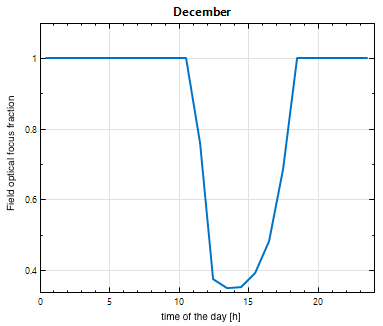
\includegraphics[width=1\textwidth]{FIG/FocusFraction/DecemberCR}
                \caption{Average CR heliostat field focus fraction in December at a SM of 3.0 and 14~h of TES.}\label{DecemberCR}
        \end{subfigure}%
        ~
        \begin{subfigure}[b]{0.5\textwidth}
                \centering
                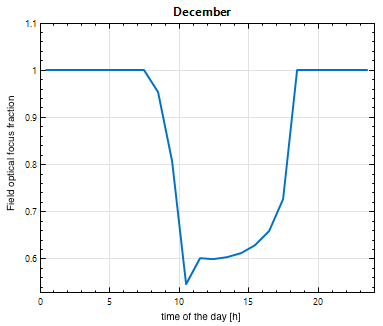
\includegraphics[width=1\textwidth]{FIG/FocusFraction/DecemberPTC}
                \caption{Average PTC SCA field focus fraction in December at a SM of 5.0 and 12~h of TES.}\label{DecemberPTC}
        \end{subfigure}
        \caption{Average field optical focus fraction in December for CSP technologies with \SI{90}{\percent} load curve coverage.}\label{FocusFraction}
\end{figure}

%The designed PV power plant is fixed orientated and doesn't track the sun, nevertheless for reaching a covering of 90~\% of the prescribed load over the first year the PV power plant needs a lower multiple of the design point than the other two solar power plants. This mainly comes from the characteristics of the PV system by using GHI instead of DNI. Upington has a huge amount on direct irradiation but also cloudy days with diffuse irradiance (see Figure~\ref{DHI-DIF}). Therefrom the PV power plant needs a lower multiple of the PV system and a smaller storage compared to the CSP power plants. Also the surplus net output of the simulated PV power plants is just about 2.2 and 5.5~\% over the year. Compared with the defocused solar field capacities of the CSP plants this is a very small value.

Although the \ac{PV} plant has fixed orientation, it needs a lower multiple of the design point than the other two solar power plants to achieve the target coverage. This is primarily due to the characteristics of the \ac{PV} system, which make better use of \ac{GHI}. Upington has strong direct irradiation but also some cloudy days with diffuse irradiance, so the \ac{PV} plant needs a lower system multiple and smaller storage compared to the \ac{CSP} plants. Surplus net output of the simulated \ac{PV} power plants is just \SIrange{2.2}{5.5}{\percent} over the year. This is very small compared to the defocused solar field capacities of the \ac{CSP} plants.


\begin{figure}[htbp]  
\centering
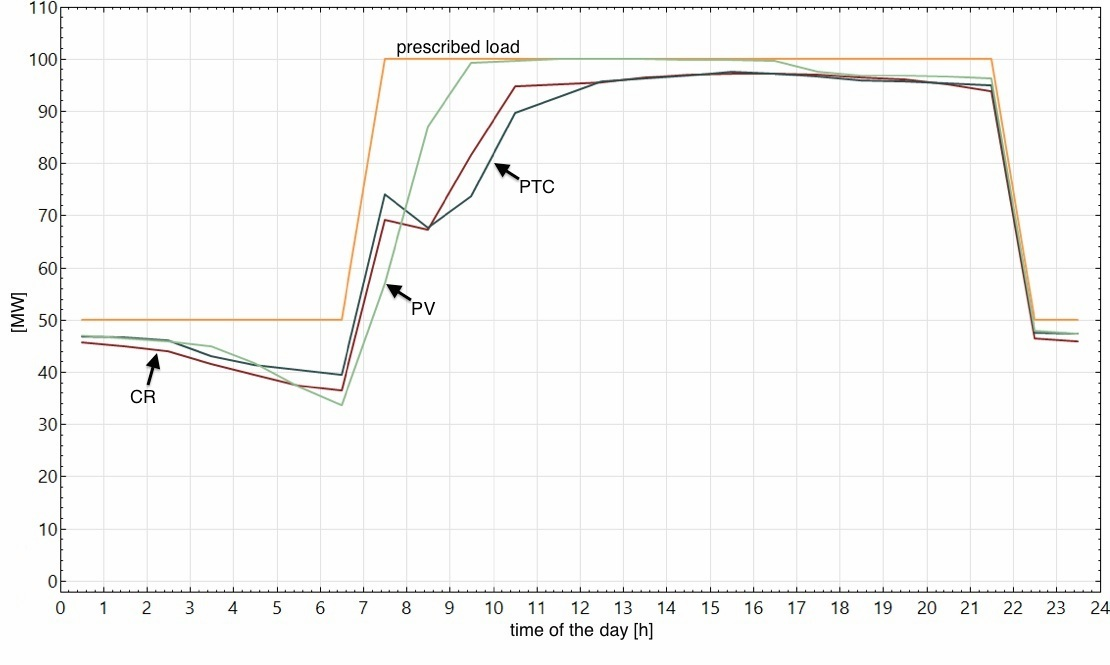
\includegraphics[width=0.9\linewidth]{FIG/90_annual_profil}
\caption{Annual average load profile of selected PV power plant configurations.}\label{90_annual_profil}
\end{figure}
%The annual average load profiles of the in Table~\ref{tbl: summaryresult} specified  power plant configuration over 90~\% load covering are compared in Figure~\ref{90_annual_profil}. It can be seen that they profiles of the three solar power plant are relatively equal. But it is noticeable that the PV plant can fully cover the load from 10:00 to 16:00 over the full year. Compared to are the annual average net energy outputs of the CSP plants just below, but can't cover the load like the PV power plant. This mainly comes from the not exactly configurable turbine power output control, which settings was described in the respective simulation design sections. It can be assumed that under real conditions a steam Rankine power output control is working far more accurate. 

The load profiles of the three solar power plants (Table~\ref{tbl: summaryresult}) are similar (Figure~\ref{90_annual_profil}). It is notable that the \ac{PV} plant can fully cover the load from 10:00 to 16:00 over the full year. In contrast, the annual average net energy outputs of the \ac{CSP} plants cannot completely cover the load. This is mainly the result of limited turbine power output control, which settings were described in the respective simulation design sections. Under real conditions, a steam Rankine power output control would be far more accurate. 

%As the line chart shows all simulated solar power plants are having there main leak in supply during the morning hours. But this mainly comes from the weaker power generation during the winter time, where the irradiation amount and angle of sunlight radiation is lower. Basically can be said that all three here shown solar power plant covers the load almost continuously over the year, but during the mentioned time during the winter all solar power plants coming to standstill. This can also be seen in the net power output heat maps of Figure~\ref{Heatmap}. The Figures describes the net power output of the selected simulated solar power plants at any hour of the simulated year. It just shows the net power output which is covering  the prescribed load and no surplus net power. It describes therefore the values of the annual average load profile from the line chart above more in detail. The power reduction during the night time from 22:00 to 7:00 is clearly visible in the heat maps. Also can be seen, that all solar power plants has interruptions in supply on various days in the year which leads from low direct or global irradiation at days of bad weather. 

All the simulated plants have loss of supply during the morning hours. This is caused mainly by weaker power generation during winter, where irradiation and sun angle are lower. All three plants cover the load almost continuously over the year, except during the late morning hours. The power output heat maps (Figure~\ref{Heatmap}, page~\pageref{Heatmap}) illustrate the net power output of the selected simulated solar power plants at any hour of the simulated year. These heat maps show only the net power output covering the prescribed load and ignore any surplus. The power reduction during the interval from 22:00 to 7:00 is clearly visible in the heat maps. Also apparent are interruptions in supply resulting from low direct or global irradiation on bad weather days. 

\begin{figure}[!htbp]
        \centering   
        \begin{subfigure}[b]{1\textwidth}
                \centering
                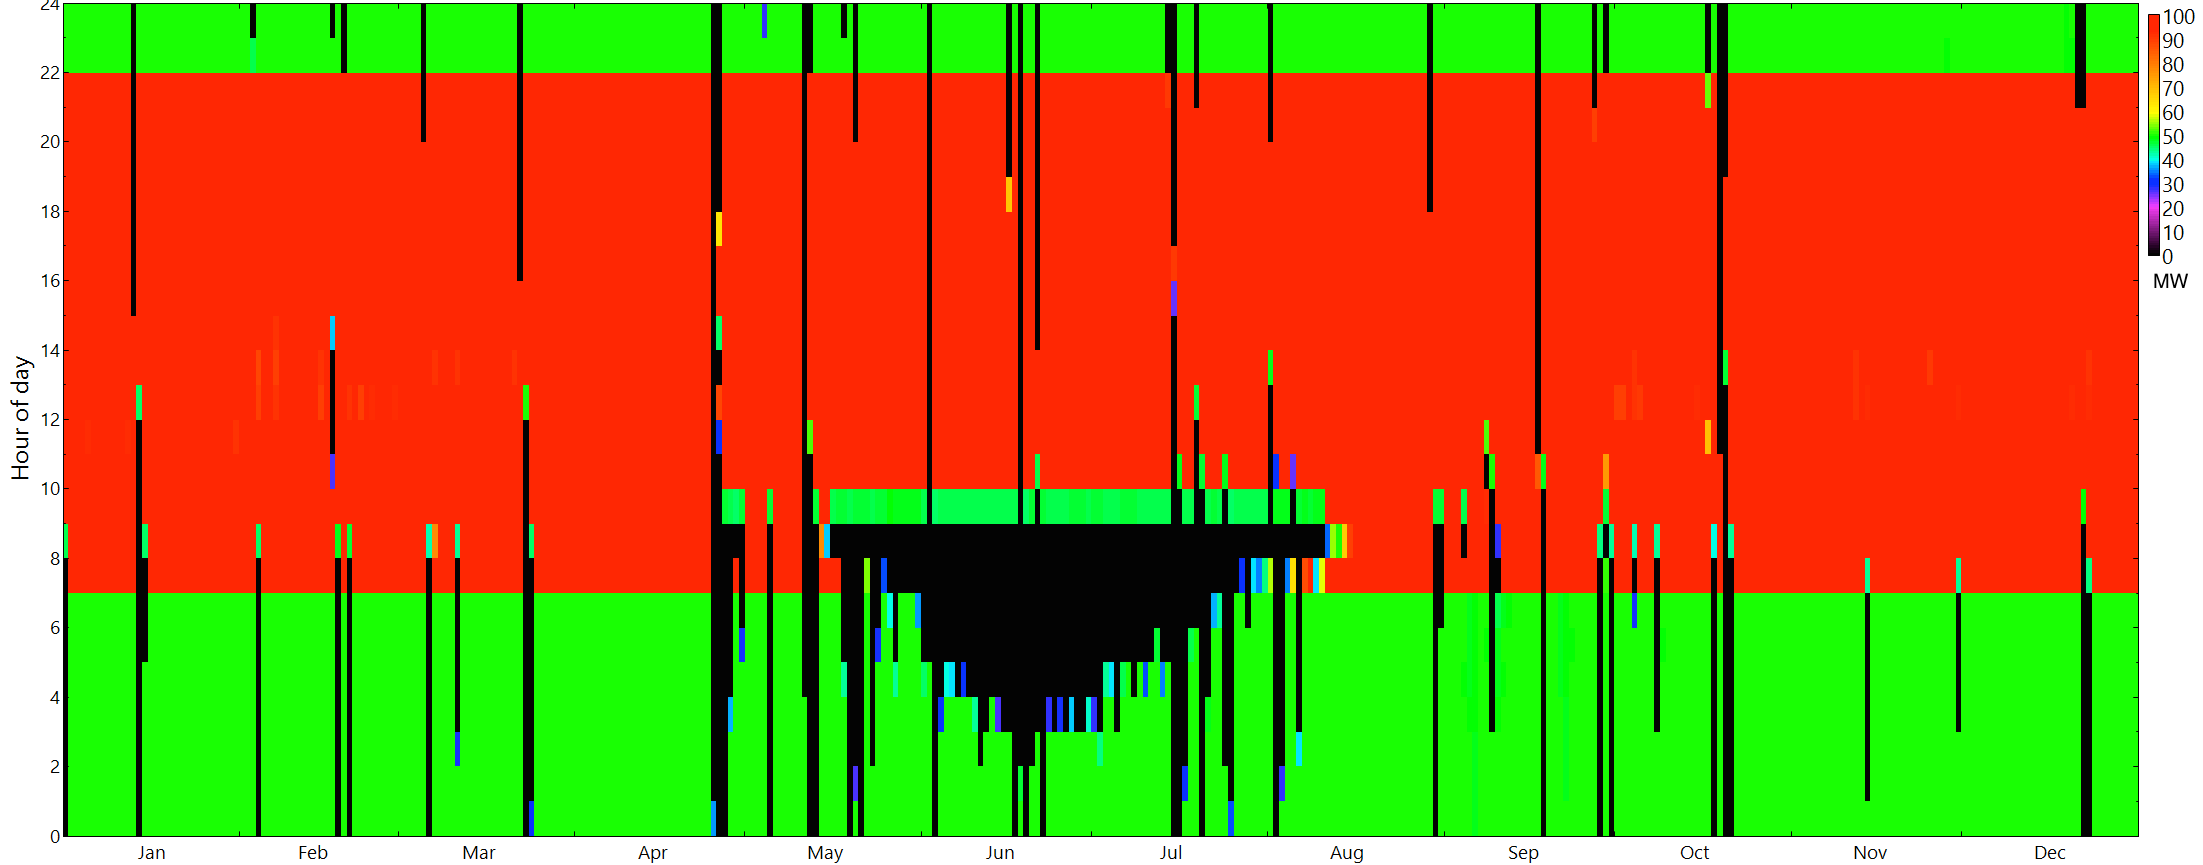
\includegraphics[width=1\textwidth]{FIG/HeatmapCR}
                \caption{CR with a SM of \num{3.0} and \SI{14}{h} TES.}\label{HeatmapCR}
        \end{subfigure}
        
\par\medskip % Linebreak

        \begin{subfigure}[b]{1\textwidth}
                \centering
                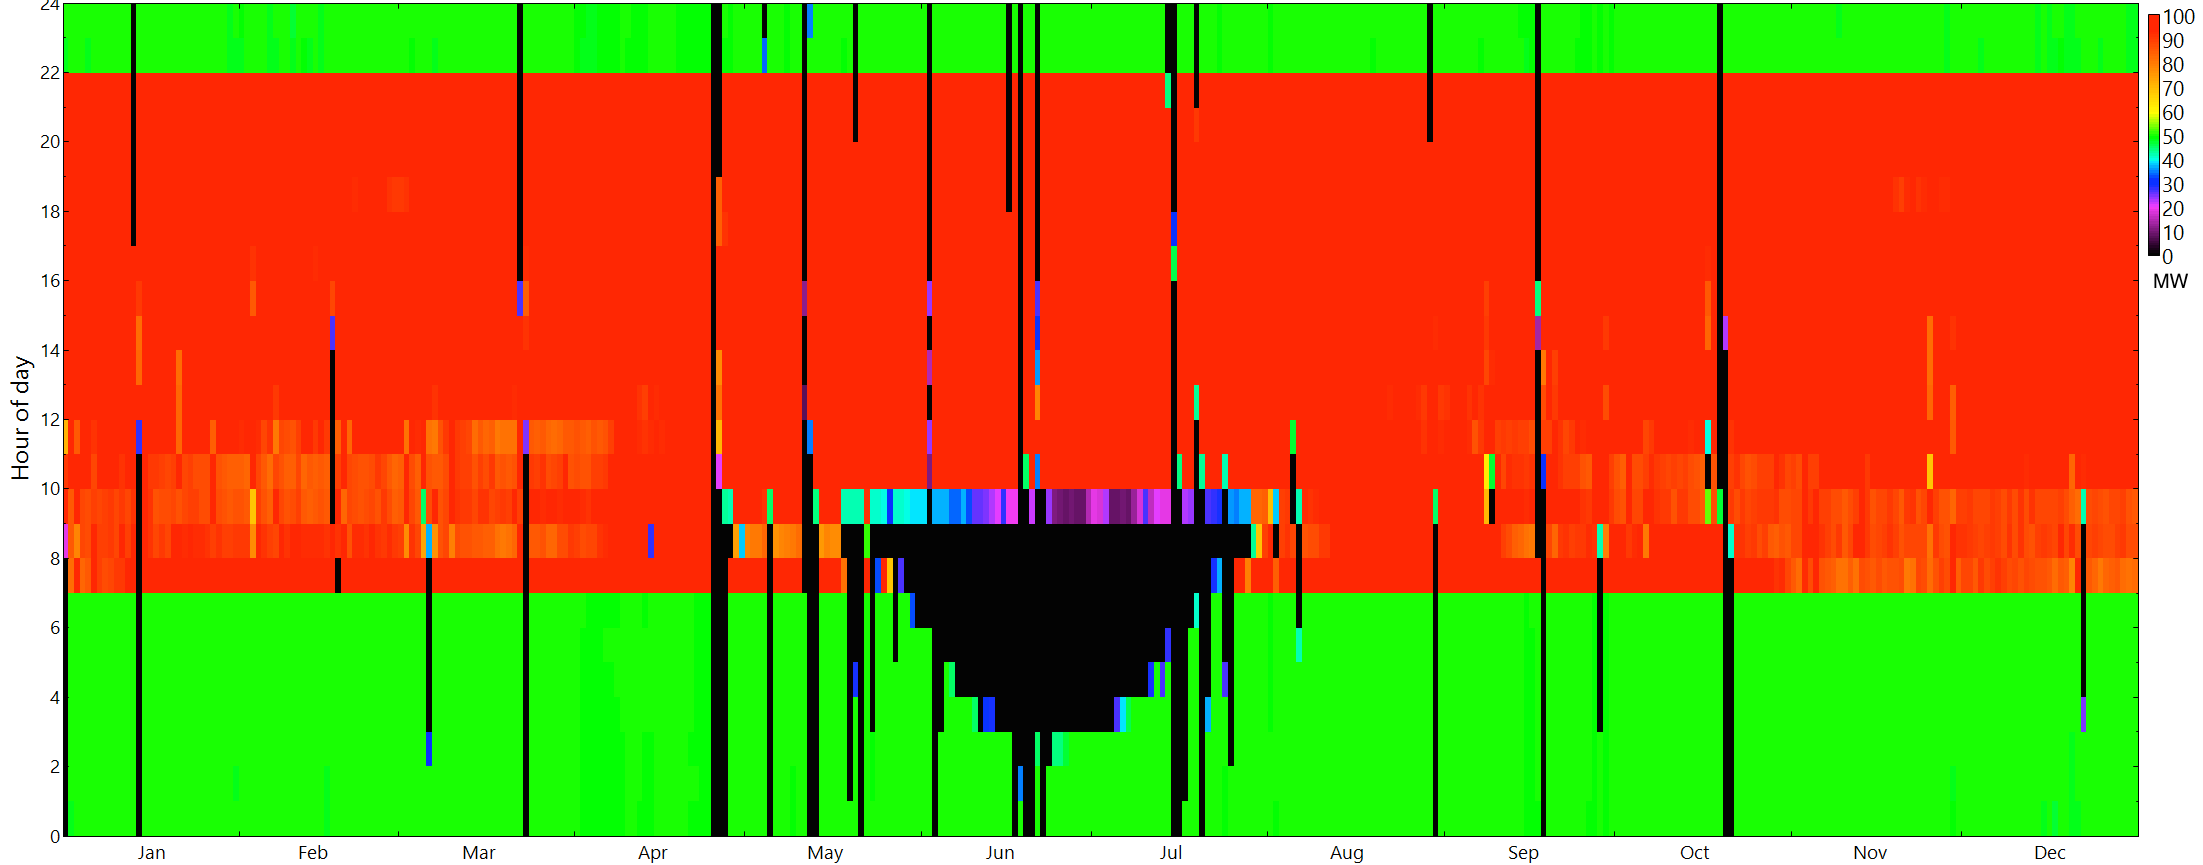
\includegraphics[width=1\textwidth]{FIG/HeatmapPTC}
                \caption{PTC with a SM of \num{5.0} and \SI{12}{h} TES.}\label{HeatmapPTC}
        \end{subfigure}
        
\par\medskip % Linebreak     
           
        \begin{subfigure}[b]{1\textwidth}
                \centering
                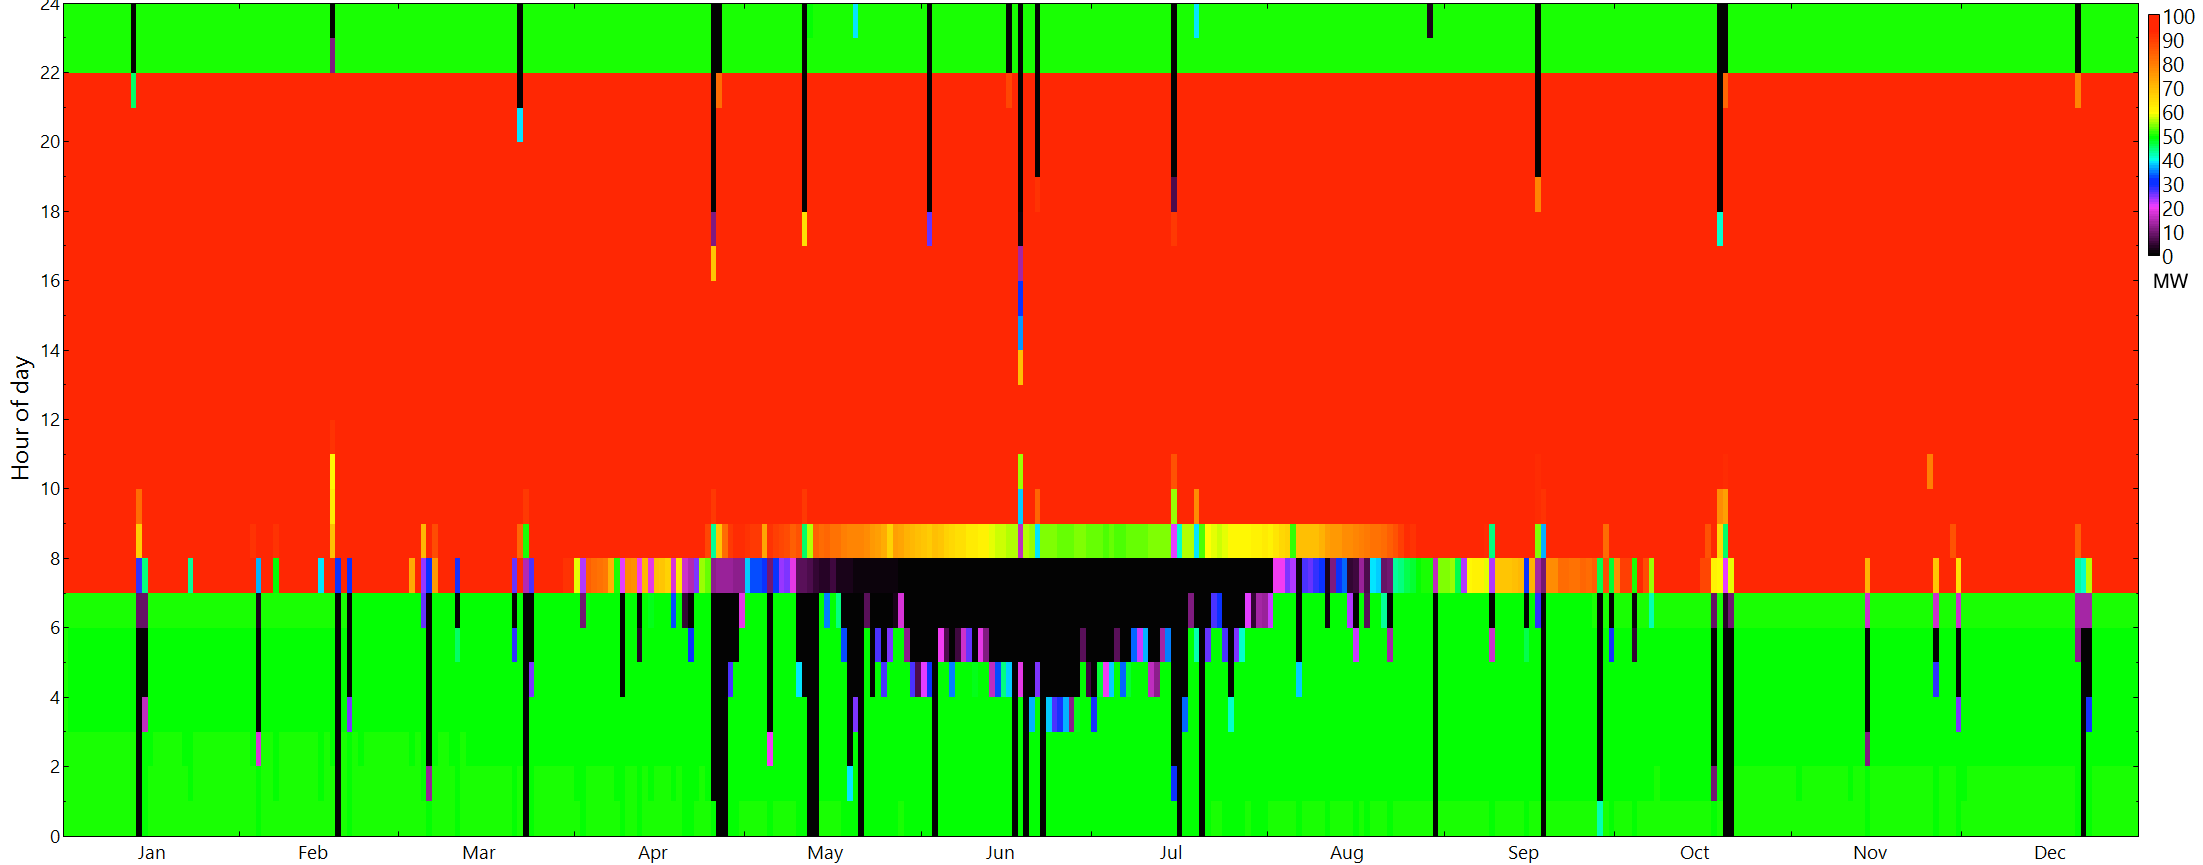
\includegraphics[width=1\textwidth]{FIG/HeatmapPV}
                \caption{PV with a PVM of \num{2.8} and \SI{7}{h} EES.}\label{HeatmapPV}
        \end{subfigure}
        \caption{Net power output to predicted load from selected solar power plants shown as heat map over the simulated year.}\label{Heatmap}
\end{figure}

%At first it is obviously when comparing the heat maps that at the time of winter solstice all power plants coming to standstill in the morning hours. When taking a view at the stating time of the power plants during that time it can be noted that the PV power plant starts about one hour earlier than the other two plants. On one site this leads from the for the PV system usable diffuse share of the GHI at dawn and on the other site from the set power block starting up time of 30 minutes for both CSP plants. It can also be noted, that the PTC system is starting with less power output then the CSP system at these time of the year.

Around the northern solstice, all power plants stop producing in the morning hours. The \ac{PV} power plant restarts about one hour earlier than the other two plants. This is partly due to the \ac{PV} plant's ability to make better use of \ac{GHI} at dawn, and partly power block start-up delay of 30 minutes for both \ac{CSP} plants. The \ac{PTC} system starts with lower power output than the \ac{CSP} system during this time of year.

%The heat map of the PTC shows a slightly lower power output during the time from 8:00 to 12:00 in summer time. This leads from the above mentioned power output control, but also from high parasitic consumer of the power plant during that time. When taking an eye on the power output of the PV power plant it can be said that the plant fully covers the predicted load over the year from 11:00 to 13:00.

The heat map of the \ac{PTC} shows a slightly lower power output during the time from 8:00 to 12:00 in summer. This results from the aforementioned power output control, but also from high parasitic load of the plant during that time. The PV power plant fully covers the predicted load over the year from 11:00 to 13:00.
\pagebreak
\section{Electricity cost results and outlook}
%The comparison shows that all solar power plants are able to cover the predicted load with there individual configured systems. But the cost effort is different between the systems which is also reflected in the investment costs and therefrom in the LCOE. Figure~\ref{LCOEcomparision} summarizes the the LCOE calculation results of the selected solar power plants from Table~\ref{tbl: summaryresult} and compares them with each other and with public projection ranges. 

The comparison shows that all solar power plants are able to cover the predicted load when configured appropriately. However, the required investment can differ substantially, which is also reflected in the capital costs and the \ac{LCOE}. Figure~\ref{LCOEcomparision} summarizes the \ac{LCOE} of the selected solar power plants from Table~\ref{tbl: summaryresult} and compares them with each other and with published projections.

%Overall for all simulated solar power plants can be said, that with the higher load covering rate also the LCOE increases.

For the simulations evaluated here, it may be said that \ac{LCOE} increases with load curve coverage.

\begin{figure}[htbp]  
\centering
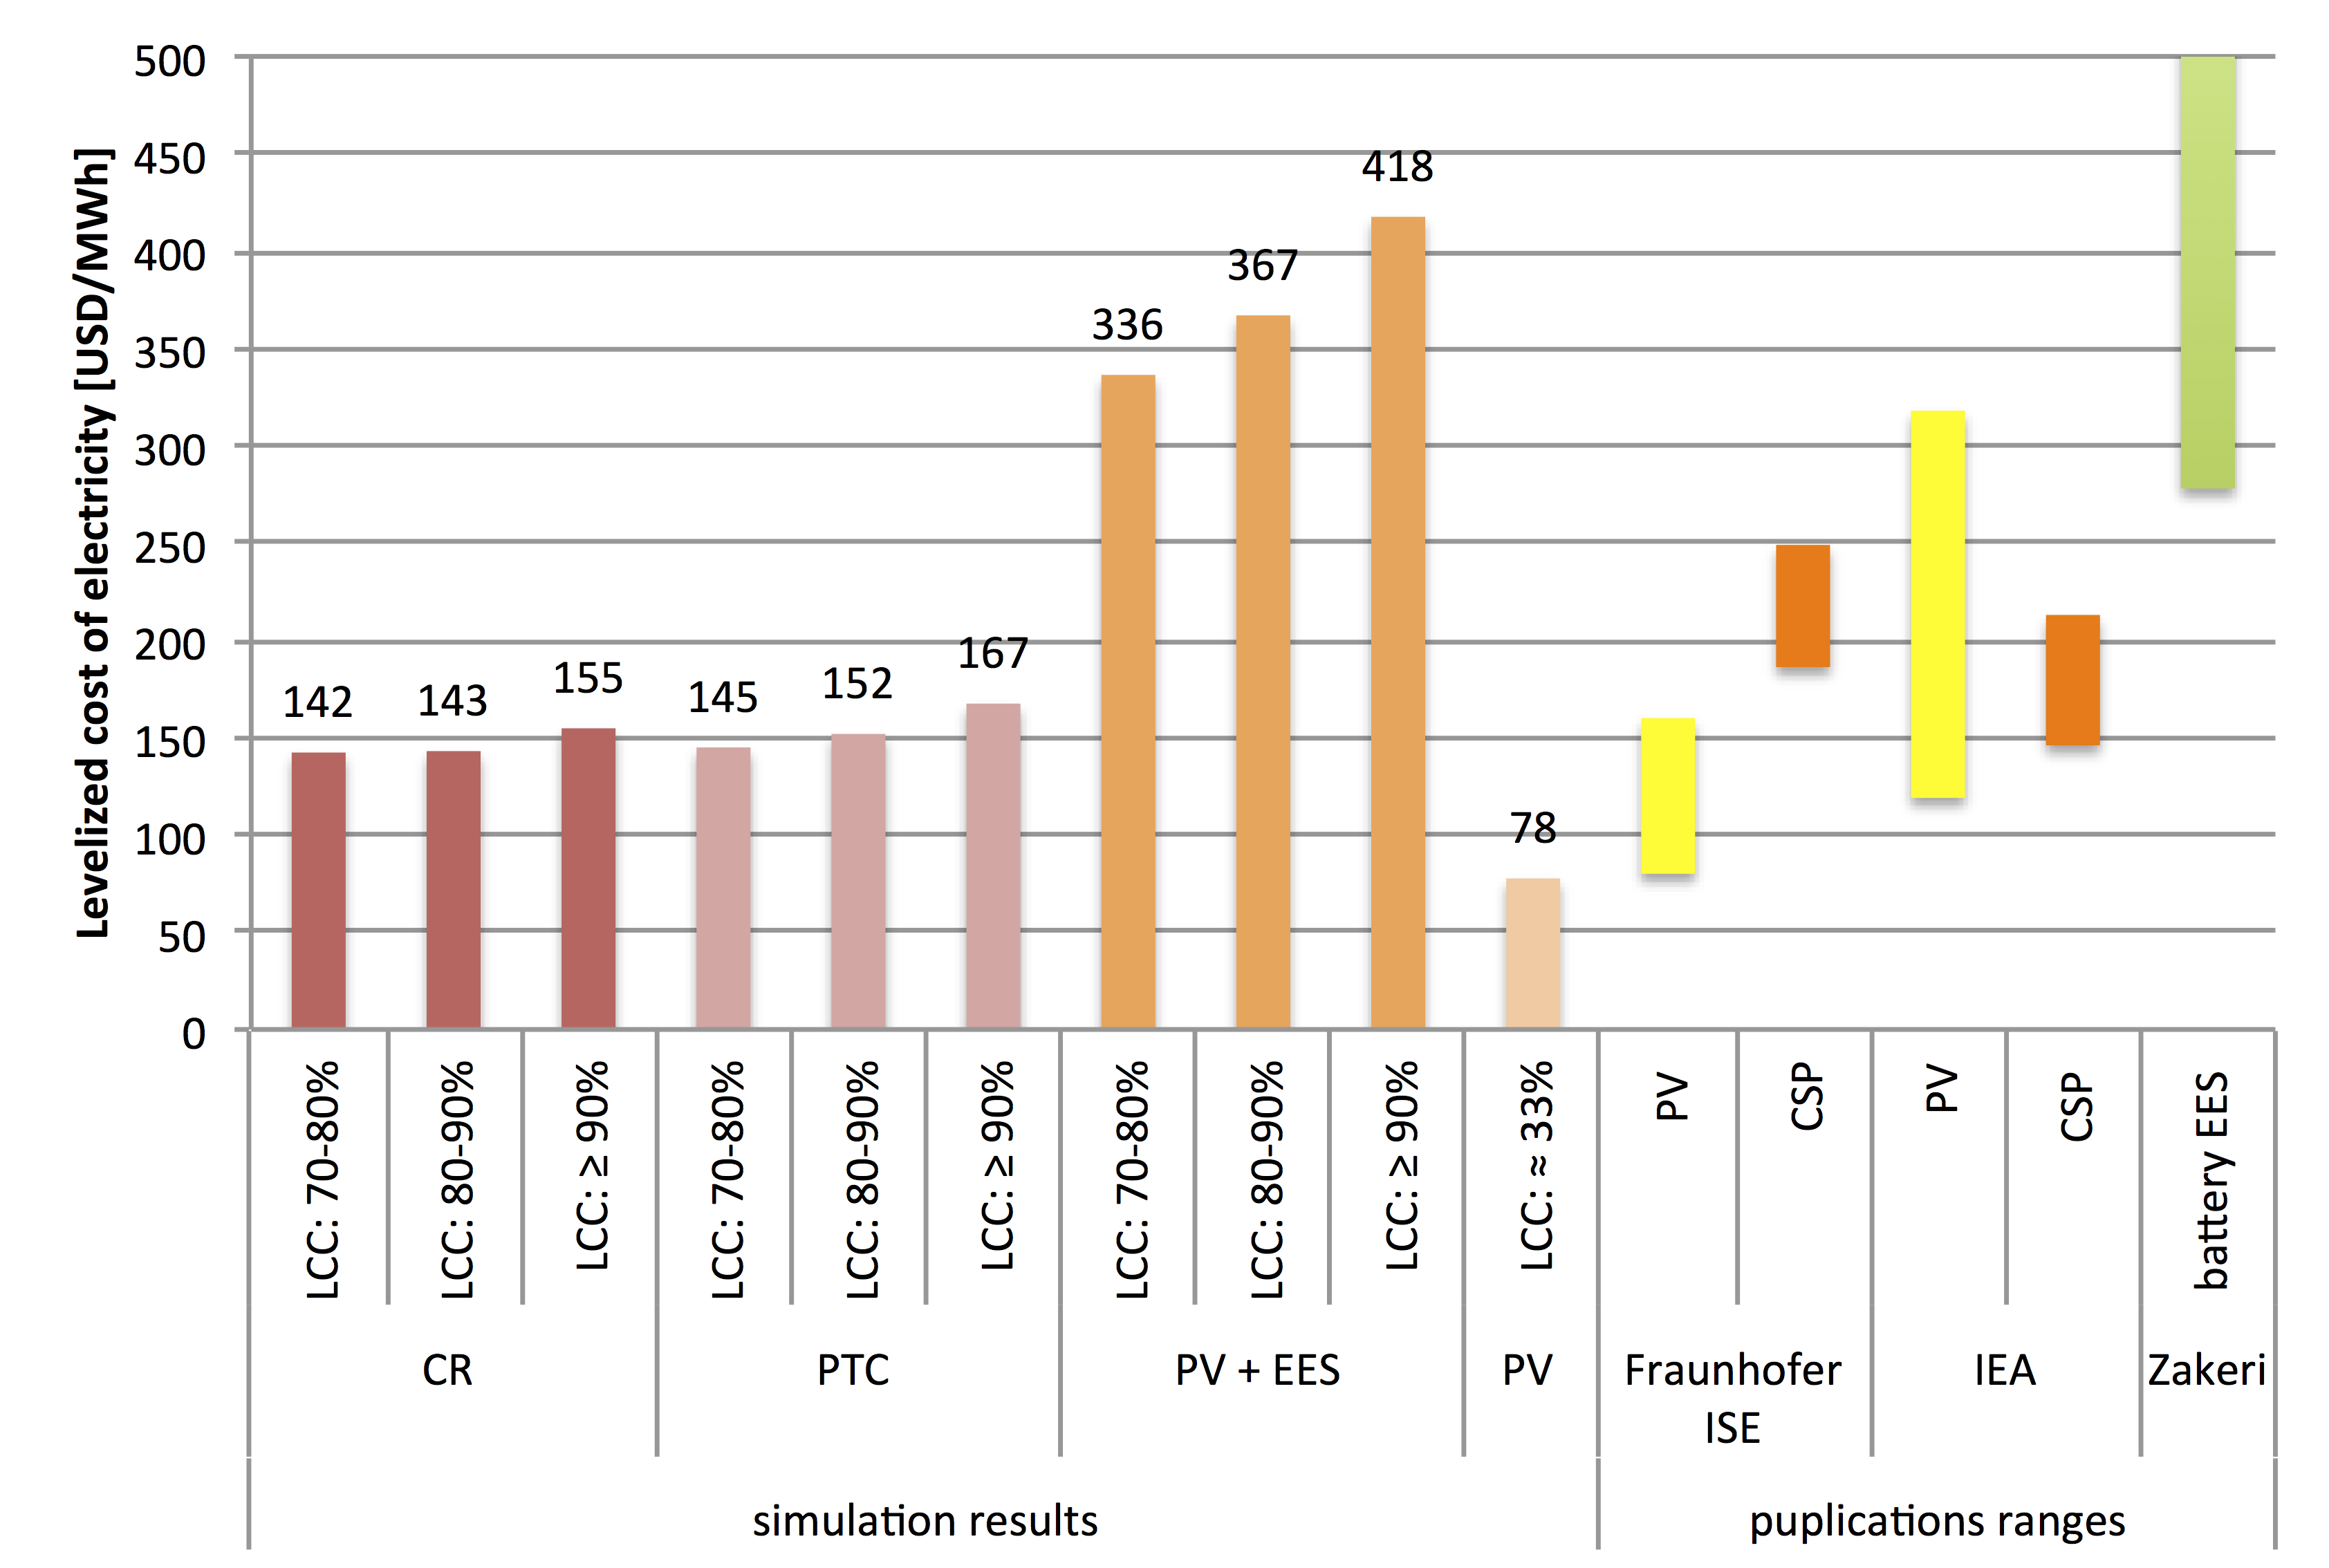
\includegraphics[width=1\linewidth]{FIG/LCOEcomparision}
\caption{Summary of calculated LCOE results of simulated solar power plants compared with public projections.}\label{LCOEcomparision}
\end{figure}
%It can be seen that the PV system without EES reaches with \SI{78}{USD/MWh} the lowest LCOE of the simulated power plants, but therby it covers the load curve just about \SI{33}{\percent} over the first year. In comparison with other projections can be seen that the PV system in Upington reaches an low LCOE result. The Fraunhofer ISE institute names the LCOE range\footnote{PV system LCOE result rages from \SIrange{60}{120}{EUR/GWh} by using a WACC of \SI{4.7}{\percent}  \cite{FraunhoferISE2013} at an avarage exchange rate in 2013 and 2014 of \SI{1.33}{USD/EUR} \cite{StatistaGmbH2015}.} for PV systems in 2013 between 80 and \SI{160}{USD/GWh} for areas with a GHI of \SIrange{1450}{2000}{\kilo\watt\hour\per\square\metre\per\year} \cite{FraunhoferISE2013}. When including the higher GHI value of Upington (\SI{2280}{\kilo\watt\hour\per\square\metre\per\year}) and the lower assumed invest costs than in 2013 the calculated LCOE seams realistic. The International Energy Agency (IEA) published the LCOE values for the year 2015 in there annual report of "Tracking Clean Energy Progress 2014" more conservative \cite{IEA2014c}.

The \ac{PV} system without \ac{EES} achieves the lowest \ac{LCOE} of the simulated power plants (\SI{78}{\usd/\mega\watt\hour}), but covers only \SI{33}{\percent} of the load curve in the first year. In comparison with other projections, the \ac{PV} system in Upington has a low \ac{LCOE}. The Fraunhofer ISE institute estimates the \ac{LCOE} range\footnote{\ac{PV} system \ac{LCOE} ranges from \SIrange{60}{120}{\eur/\giga\watt\hour} using a \ac{WACC} of \SI{4.7}{\percent} \cite{FraunhoferISE2013} at an average exchange rate in 2013 and 2014 of \SI{1.33}{\usd/\eur} \cite{StatistaGmbH2015}.} for \ac{PV} systems in 2013 between \num{80} and \SI{160}{\usd/\giga\watt\hour} for areas with a \ac{GHI} of \SIrange{1450}{2000}{\kilo\watt\hour\per\square\metre\per\year} \cite{FraunhoferISE2013}. When including the higher \ac{GHI} value of Upington (\SI{2280}{\kilo\watt\hour\per\square\metre\per\year}) and the lower assumed capital costs, the calculated \ac{LCOE} appears realistic. The \ac{LCOE} estimates published by the \ac{IEA} for the year 2015 in their annual report \emph{Tracking Clean Energy Progress 2014} were more conservative \cite{IEA2014c}.

%The lowest LCOE calculation results of the simulated solar power plants which covers more than \SI{90}{\percent} of the predicted load curve has the CR power plant with about \SI{155}{USD/MWh}. The CR power plant in generally reaches the lowest LCOE values while having a high load curve covering rate. Also the LCOE result of the PTC power plant is with \SI{167}{USD/MWh} relatively low. When comparing this values with the projections of Fraunhofer ISE institute from 2013 the results looking quite optimistic. But when comparing with the electricity cost range from the IEA publication the CSP simulation results seams realistic.

\begin{figure}[htbp]
        \centering                
        \begin{subfigure}[b]{0.5\textwidth}
                \centering
                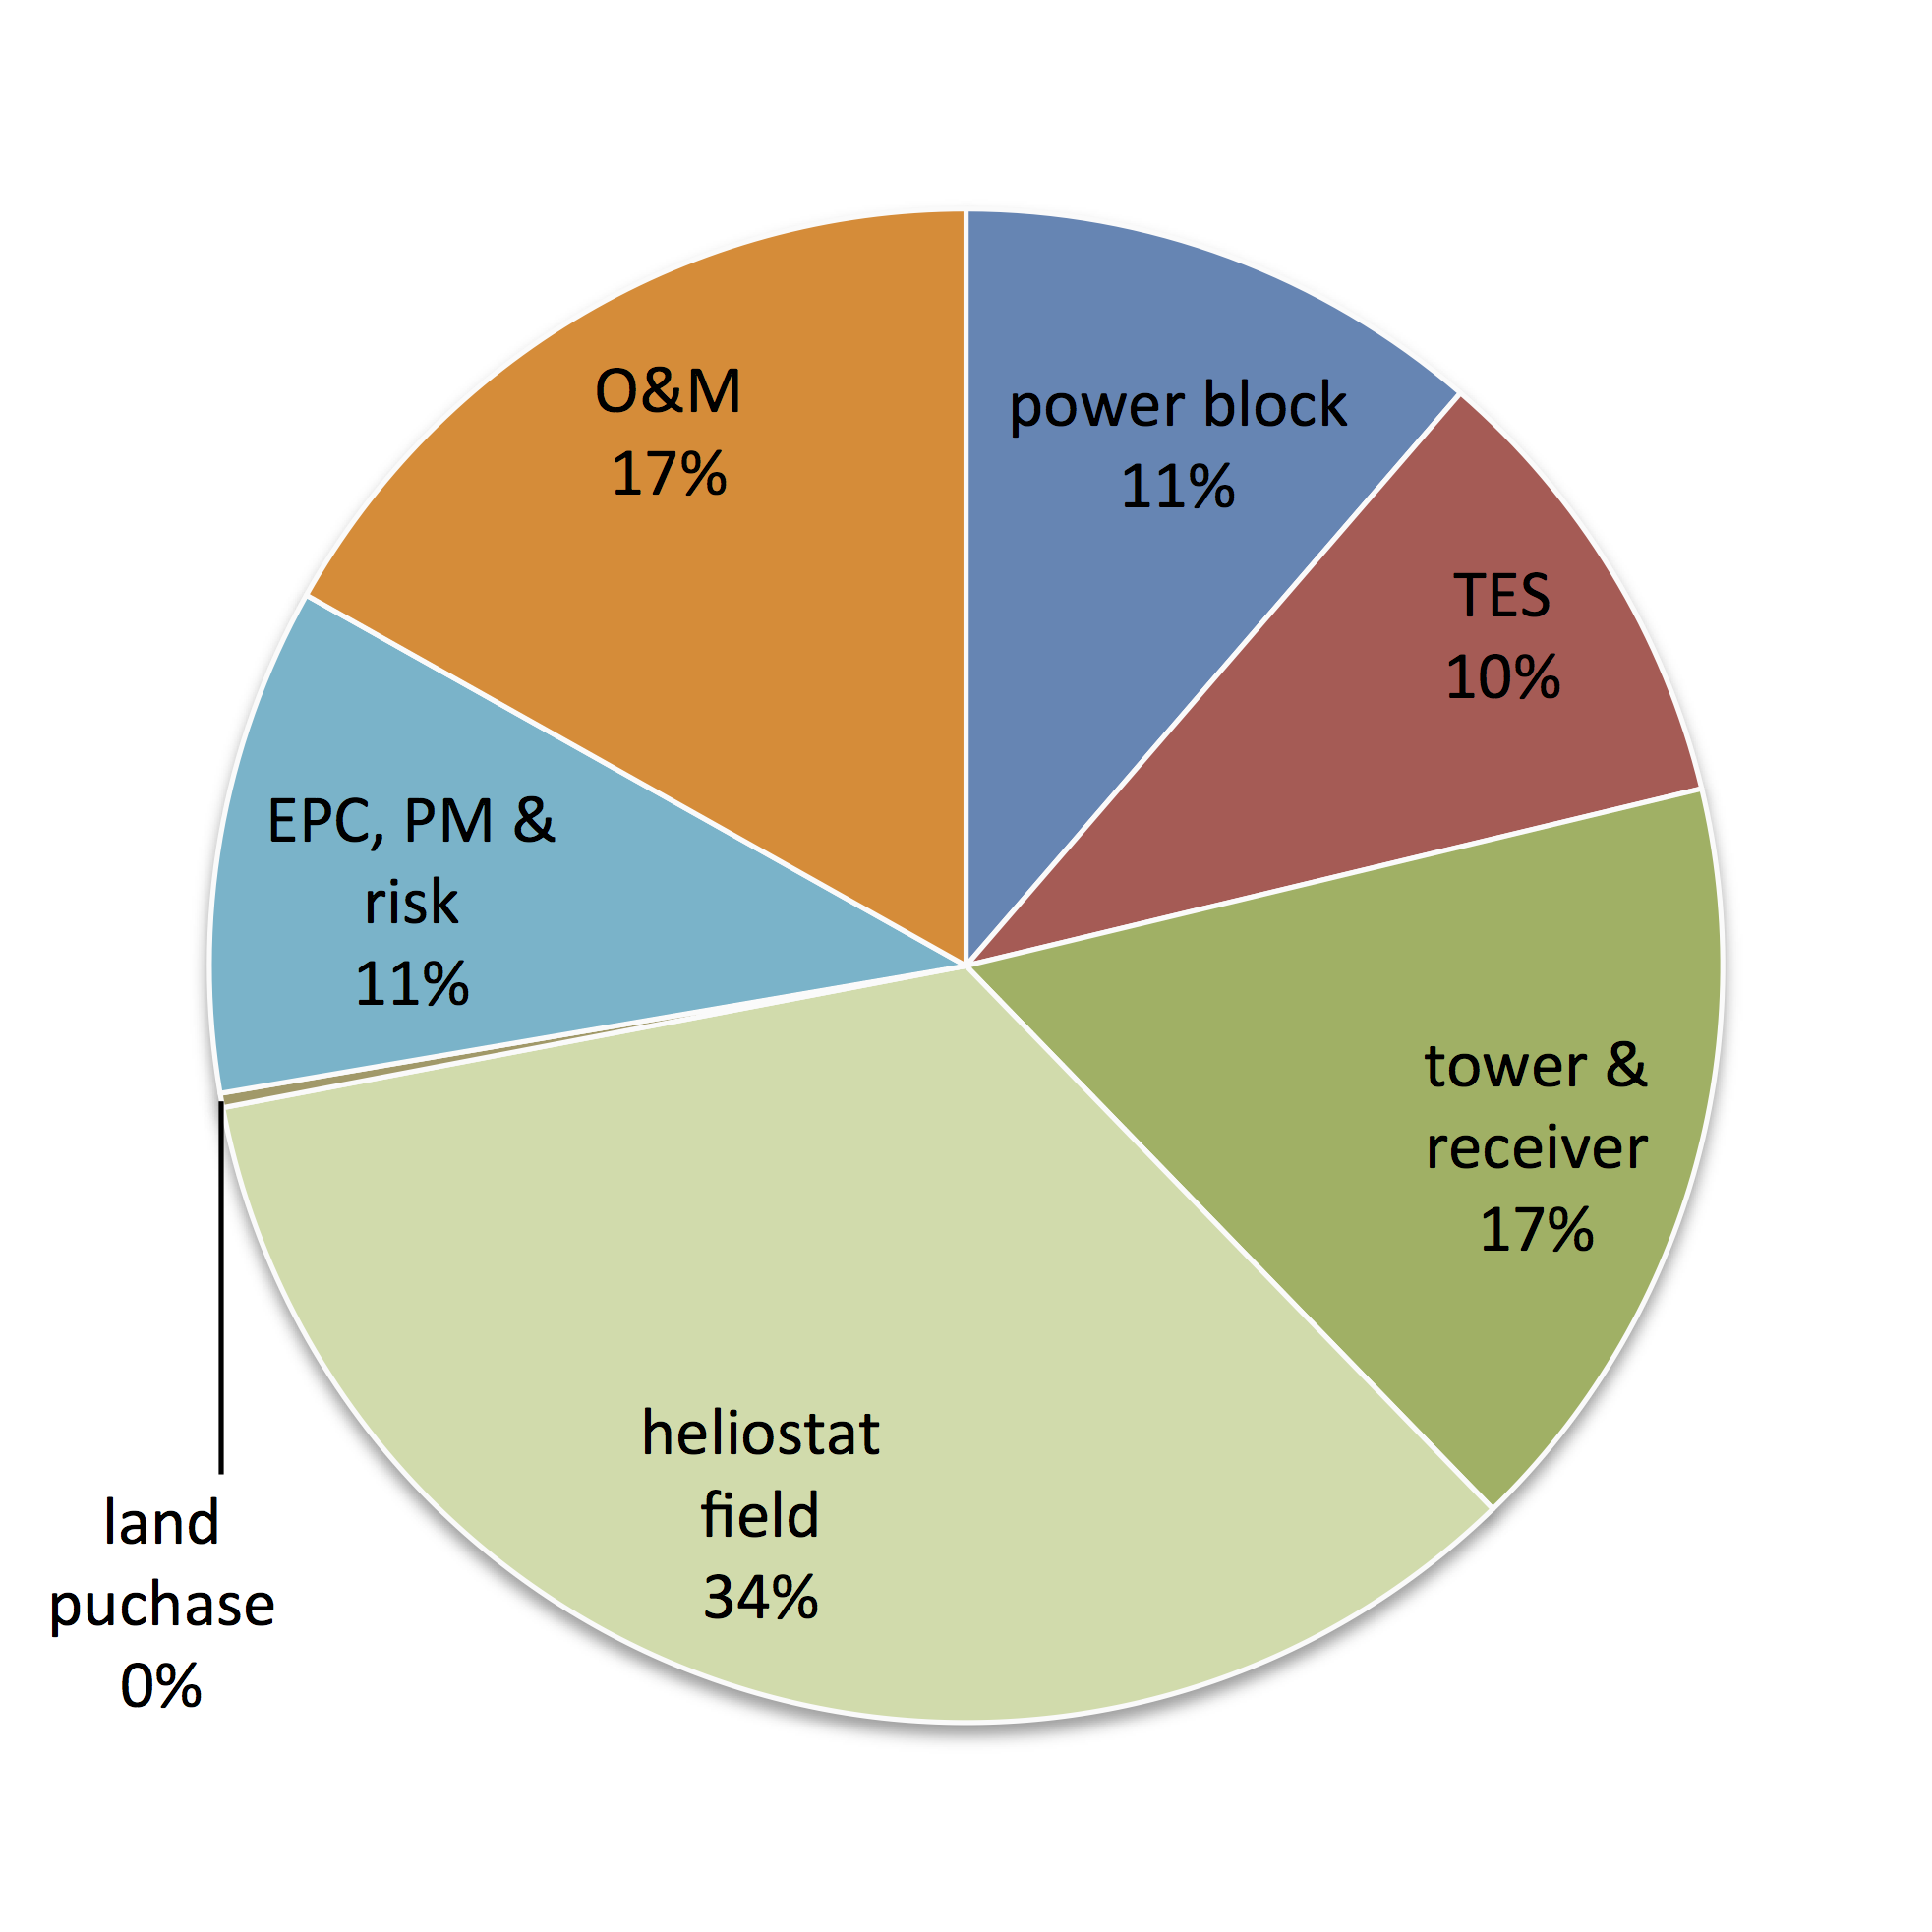
\includegraphics[width=1\textwidth]{FIG/CR_LCOE_90_BreakDown}
                \caption{CR at \SI{90}{\percent} LCC.}\label{CR_LCOE_90_BreakDown}
        \end{subfigure}%
        ~
        \begin{subfigure}[b]{0.5\textwidth}
                \centering
                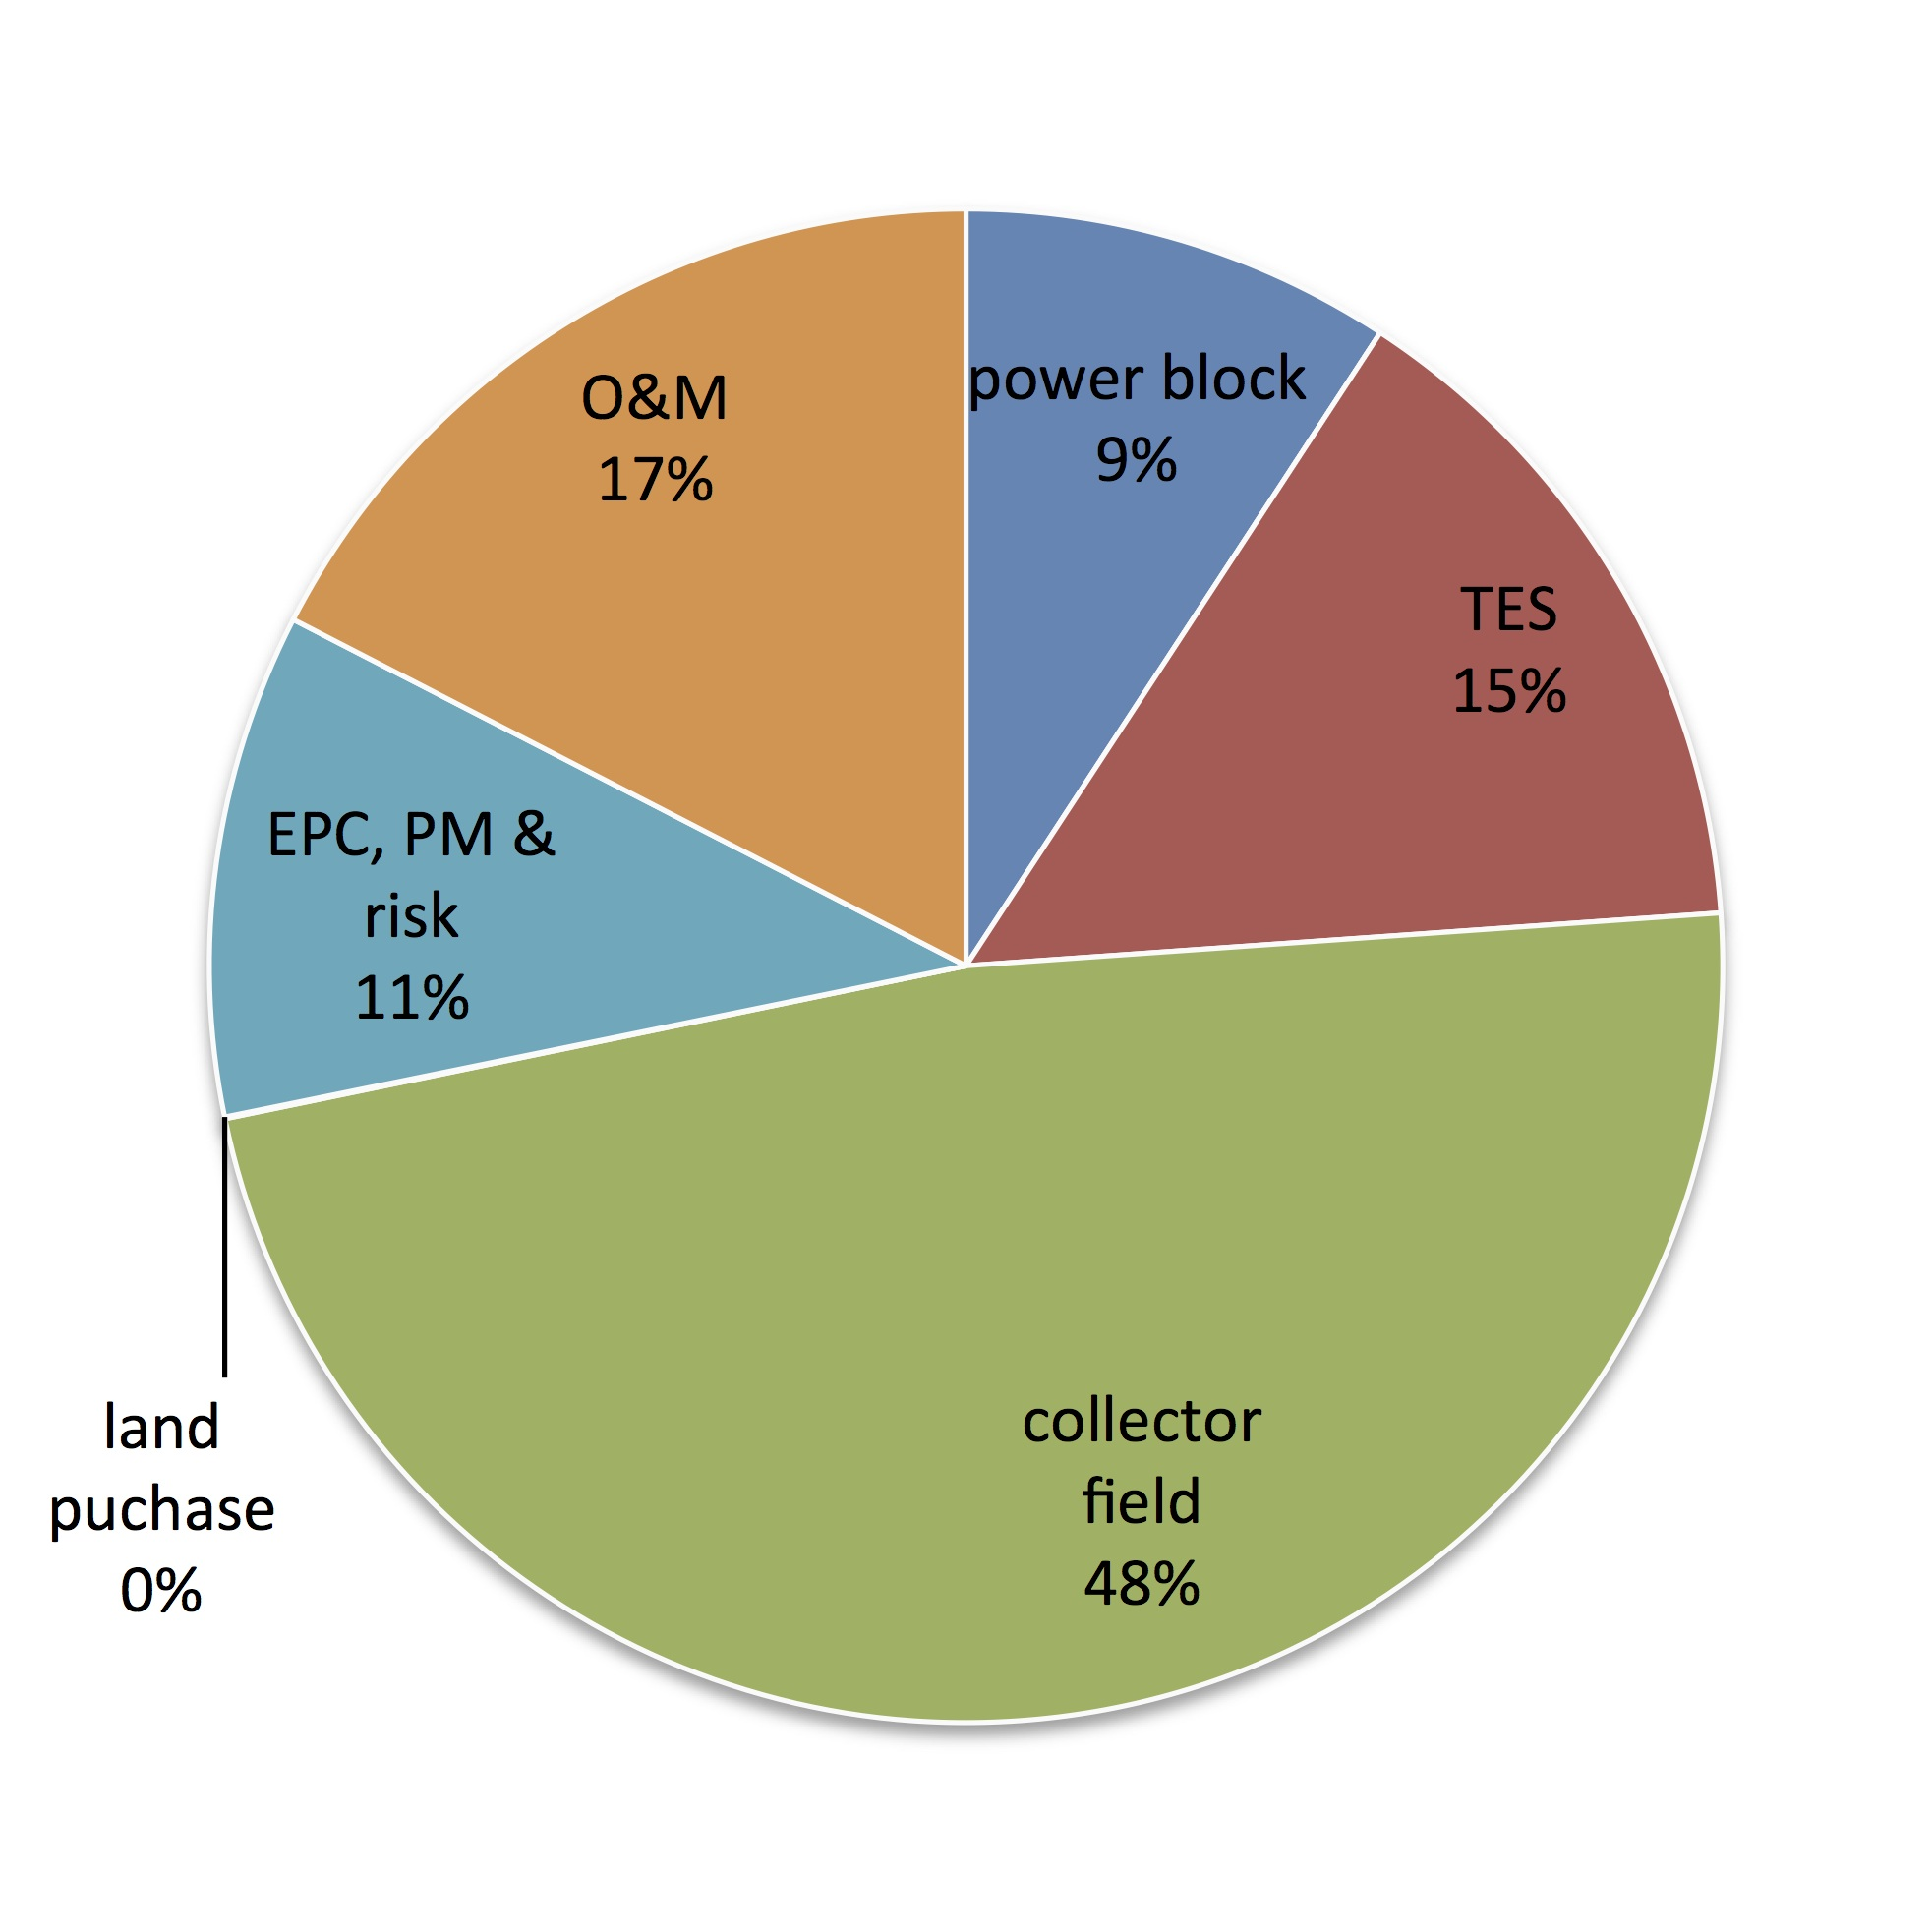
\includegraphics[width=1\textwidth]{FIG/PTC_LCOE_90_BreakDown}
                \caption{PTC at \SI{90}{\percent} LCC.}\label{PTC_LCOE_90_BreakDown}
        \end{subfigure}
\par\medskip % Linebreak   
        \begin{subfigure}[b]{0.5\textwidth}
                \centering
                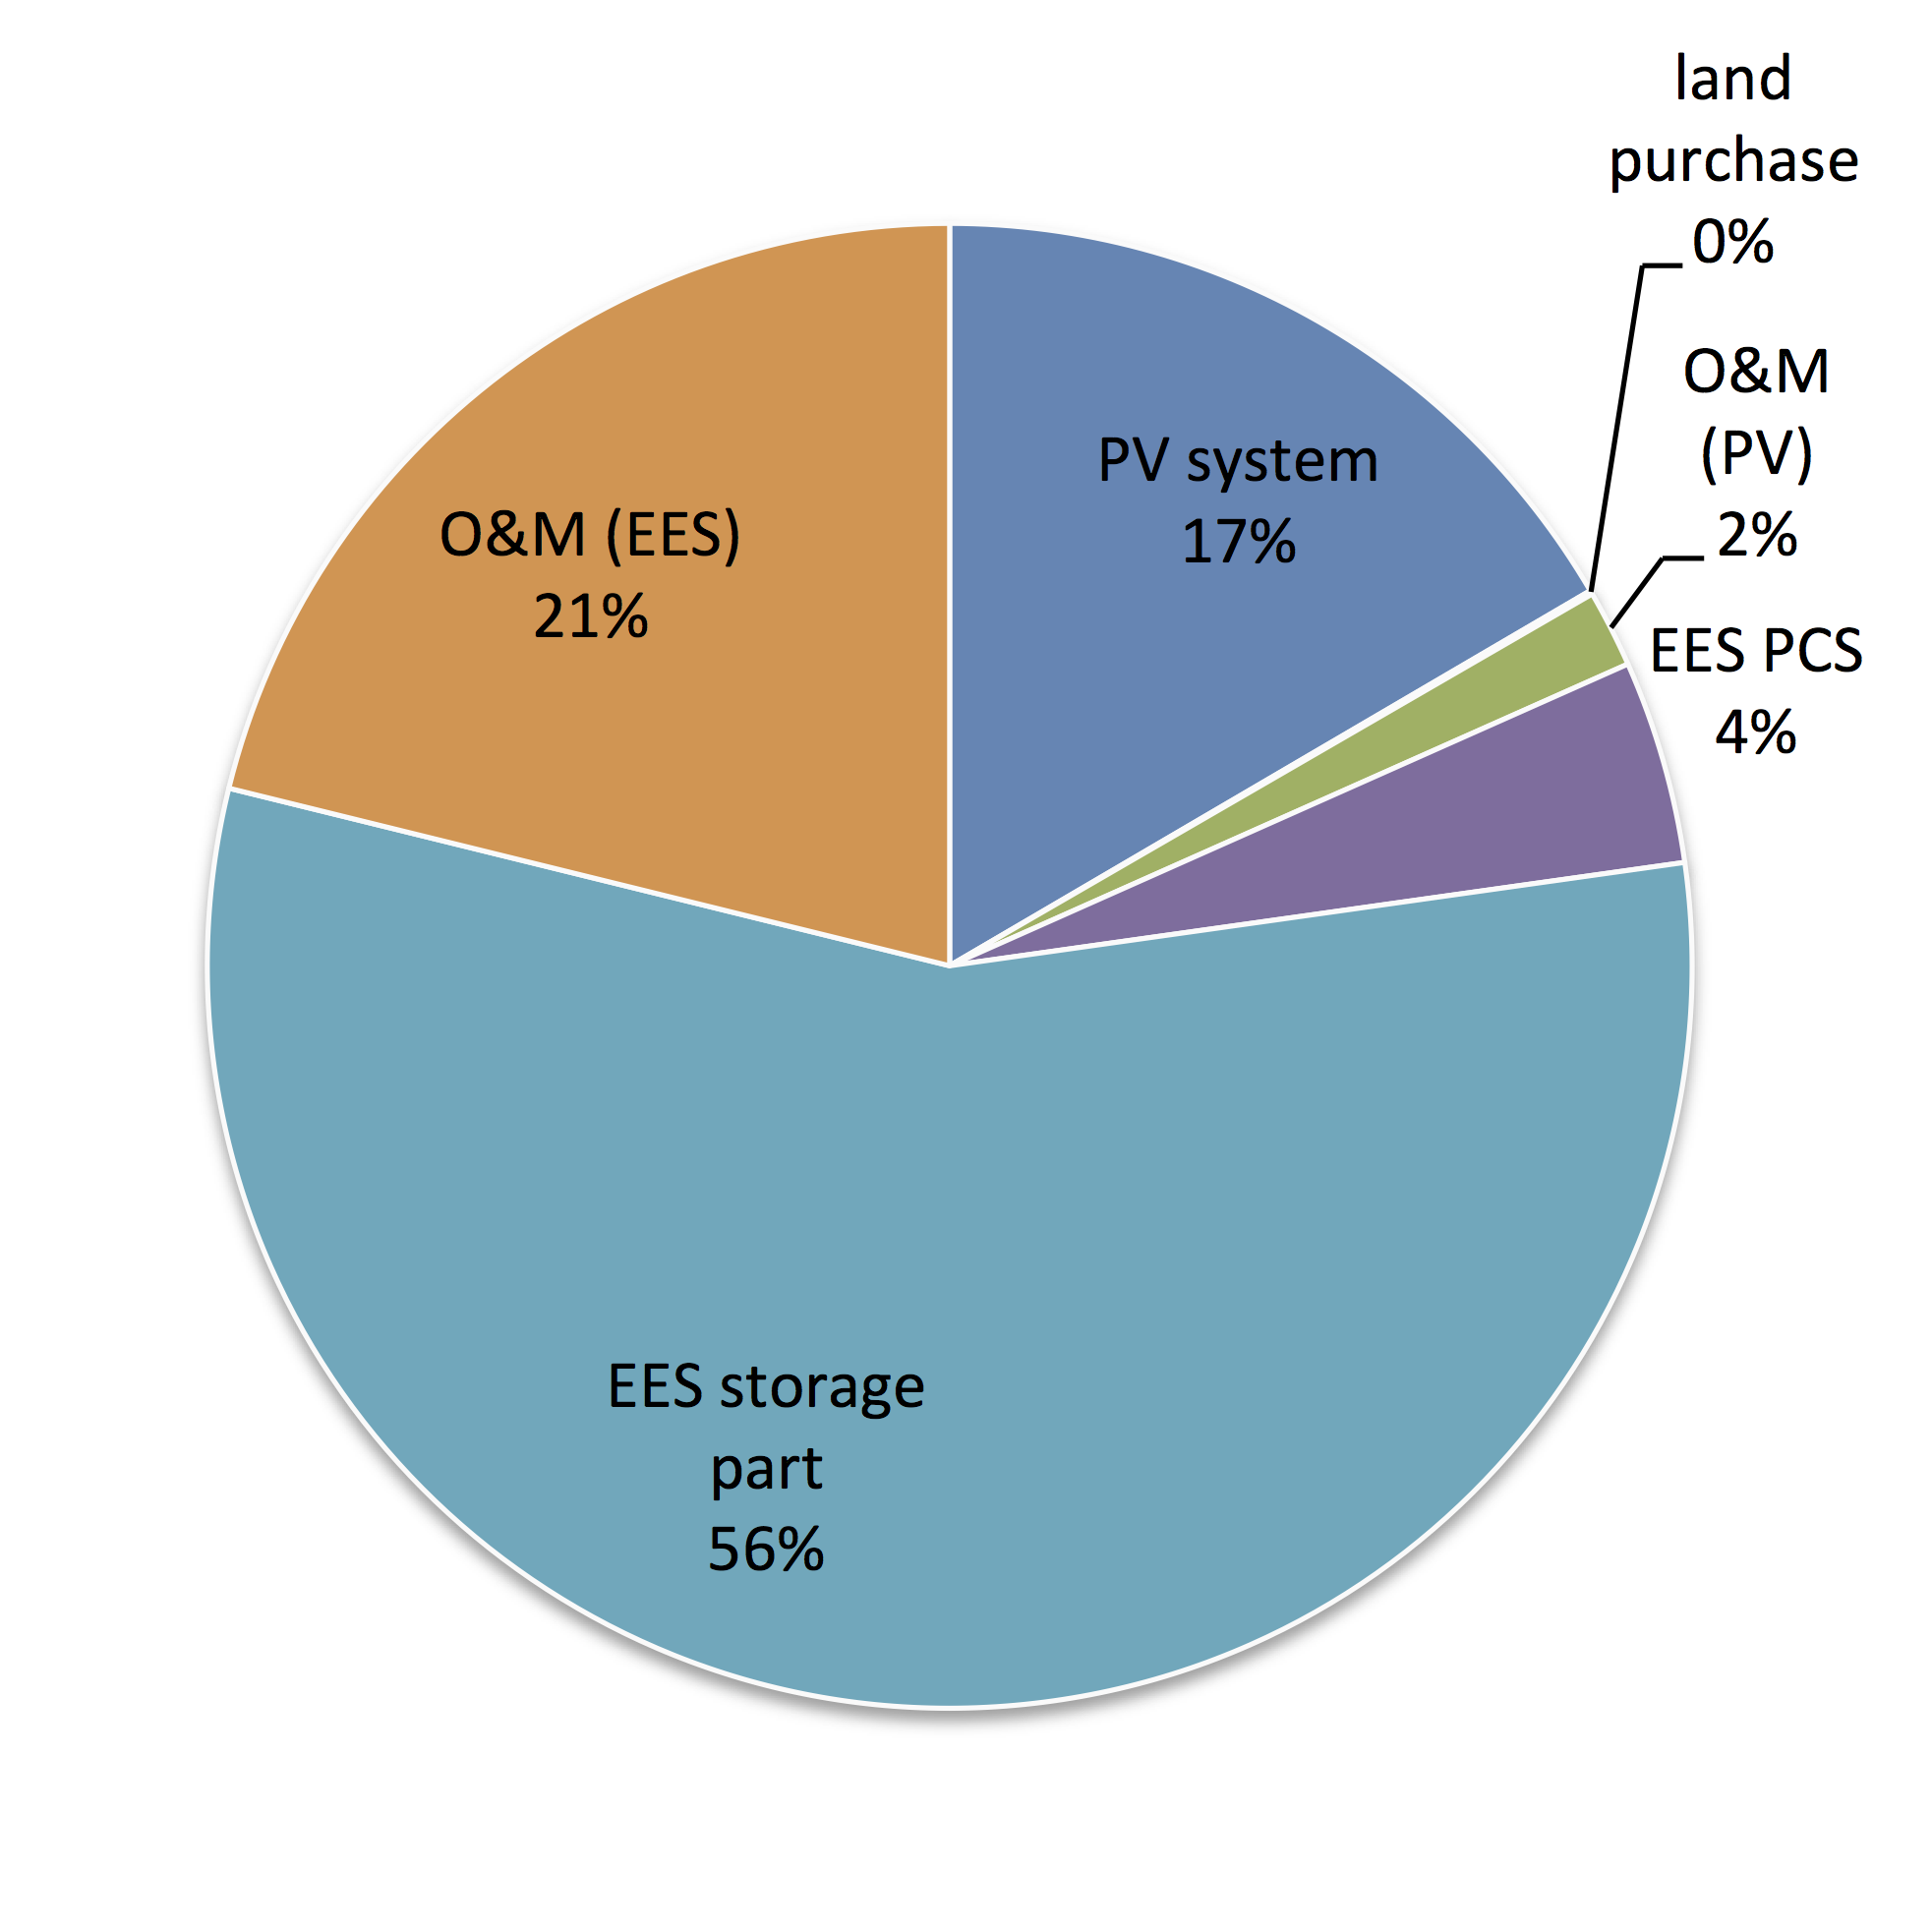
\includegraphics[width=1\textwidth]{FIG/PV_LCOE_90_BreakDown}
                \caption{PV with adapted EES at \SI{90}{\percent} LCC.}\label{PV_LCOE_90_BreakDown}
        \end{subfigure}
        \caption{Break-down of selected LCOE calculations.}\label{SMPV_LCOE_BreakDown}
\end{figure}
The lowest \ac{LCOE} for plants covering more than \SI{90}{\percent} of the predicted load curve was that of the \ac{CR} power plant, at about \SI{155}{\usd/\mega\watt\hour}. The \ac{CR} power plant reaches the lowest \ac{LCOE} values while having a high load curve coverage. The \ac{LCOE} for the \ac{PTC} power plant is also relatively low \SI{167}{USD/MWh}. These values seem optimistic when compared to Fraunhofer ISE's 2013 projections, yet again realistic when compared with \ac{IEA} projections.

%The LCOE calculation results of the simulated PV system with adapted EES is by far the most expansive solution for suppling the prescribed load. The lowest LCOE for reaching \SI{90}{\percent} LCC is more than twice that high than from the CSP options. For the comparison also must be remembered, that the costs of the EES storage part was assumed extremely low in comparison with the average marked price (Page~\pageref{SUBSUBPVFinancialparameter}). But when using other optimistic LCOE calculations of battery EES the result seams realistic. There are optimistic puplications calculated a LCOE of a battery EES with about \SI{200}{USD/MWh} pure storage costs \cite{Corcuera2015}. Also other publications can confirmed this result for EES. The range\footnote{EES sysfem LCOE result ranges from \SIrange{209}{617}{EUR/MWh} by using an energy price of \SI{50}{EUR/MWh} and \SI{8}{\percent} WACC rate \cite{Zakeri2015} at an avarage exchange rate in 2013 and 2014 of 1.33 USD/EUR \cite{StatistaGmbH2015}.} of LCOE for battery storage is named there between \SIlist{278;821}{USD/MWh}. However he results the LCOE of the Li-Ion battery at the top end.

The \ac{LCOE} of the simulated \ac{PV} system with adapted \ac{EES} is by far the most expensive solution. The lowest \ac{LCOE} at \SI{90}{\percent} \ac{LCC} is more than twice that of the \ac{CSP} designs. Note again that the assumed costs of the \ac{EES} were extremely low in comparison with the average market price (Page~\pageref{SUBSUBPVFinancialparameter}); when using other optimistic \ac{LCOE} calculations of battery \ac{EES} the result appears realistic. Optimistic projections calculated \ac{LCOE} with battery \ac{EES} assuming \SI{200}{\usd/\mega\watt\hour} pure storage costs \cite{Corcuera2015}. Other publications confirm this; the range\footnote{\ac{EES} system \ac{LCOE} ranges from \SIrange{209}{617}{\eur/\mega\watt\hour} assuming an energy price of \SI{50}{\eur/\mega\watt\hour} and \SI{8}{\percent} \ac{WACC} rate \cite{Zakeri2015} at an average exchange rate in 2013 and 2014 of \SI{1.33}{\usd/\eur} \cite{StatistaGmbH2015}.} of \ac{LCOE} for battery storage is estimated between \SIlist{278;821}{\usd/\mega\watt\hour}, with \ac{li-ion} battery storage being the most expensive.

%Comparing the LCOE break-down shares (Figure~\ref{SMPV_LCOE_BreakDown}) of the selected simulated solar power plants it shows that the CSP power plants costs are dominated by the concentrating and heat collecting components, while the main cost part of the PV power plant is the EES part. The EES makes more than \SI{80}{\percent} of the PV plants LCOE share. This is a huge share compared with the TES of the CSP plants. It can be seen that the TES of the PTC system has a greater proportion of the costs than in the CR system, which is based in the twice that high specific costs for the storage. The capital cost for land purchase are that low that they has no influence on any simulated solar power plant LCOE. 

Costs of \ac{CSP} power plants are dominated by the concentrating and heat-collecting components, while the main cost item of the \ac{PV} power plant is \ac{EES} (Figure~\ref{SMPV_LCOE_BreakDown}). The \ac{EES} makes up more than \SI{80}{\percent} of the \ac{PV} plants \ac{LCOE} share, much more than \ac{TES} in \ac{CSP} plants. The \ac{TES} of the \ac{PTC} system has a greater proportion of the costs than in the \ac{CR} system, which is a result of high specific costs for the storage. The capital costs for land purchase are so low that they have little influence on \ac{LCOE}. 
\pagebreak
%The sum of the specific investment costs of the selected CSP plants are with \SI{7503}{USD/kW} for the CR system and \SI{7540}{USD/kW} for the PTC system almost the same. This fits also to the from the IEA predicted average specific investment cost in 2015 with about \SI{7362}{USD/kW} \cite{IEA2014c}. The PV system was calculated with specific investment costs of \SI{1285}{USD/kW} (Page~\pageref{SUBSUBPVFinancialparameter}) which is below the prognosticated cost range of the IEA for large-scale solar PV systems (Figure~\ref{investmentcost}). 

Total specific investment costs of the selected \ac{CSP} plants are similar, at \SI{7503}{USD/kW} for the \ac{CR} system and \SI{7540}{\usd/\kilo\watt} for the \ac{PTC} system. This is consistent with the \ac{IEA}'s predicted average specific investment cost in 2015, which was \SI{7362}{\usd/\kilo\watt} \cite{IEA2014c}. The \ac{PV} costs were calculated using specific investment costs of \SI{1285}{\usd/\kilo\watt} (see page~\pageref{SUBSUBPVFinancialparameter}) which is below the prognosticated cost range of the \ac{IEA} for utility-scale solar \ac{PV} systems (Figure~\ref{investmentcost}). 

%The IEA gives also a prediction for solar power investment cost degradation till 2050. After this prognosis will the specific investment costs of the CSP decrease by about \SI{54}{\percent} and the PV system costs by about \SI{60}{\percent} in total till 2050 \cite{IEA2014c}.

The \ac{IEA} has also issued a prediction for solar power investment cost degression. According to this prognosis, specific investment costs of \ac{CSP} will decrease by about \SI{54}{\percent} and the \ac{PV} system costs by about \SI{60}{\percent} by \cite{IEA2014c}.

\begin{figure}[htbp]  
\centering
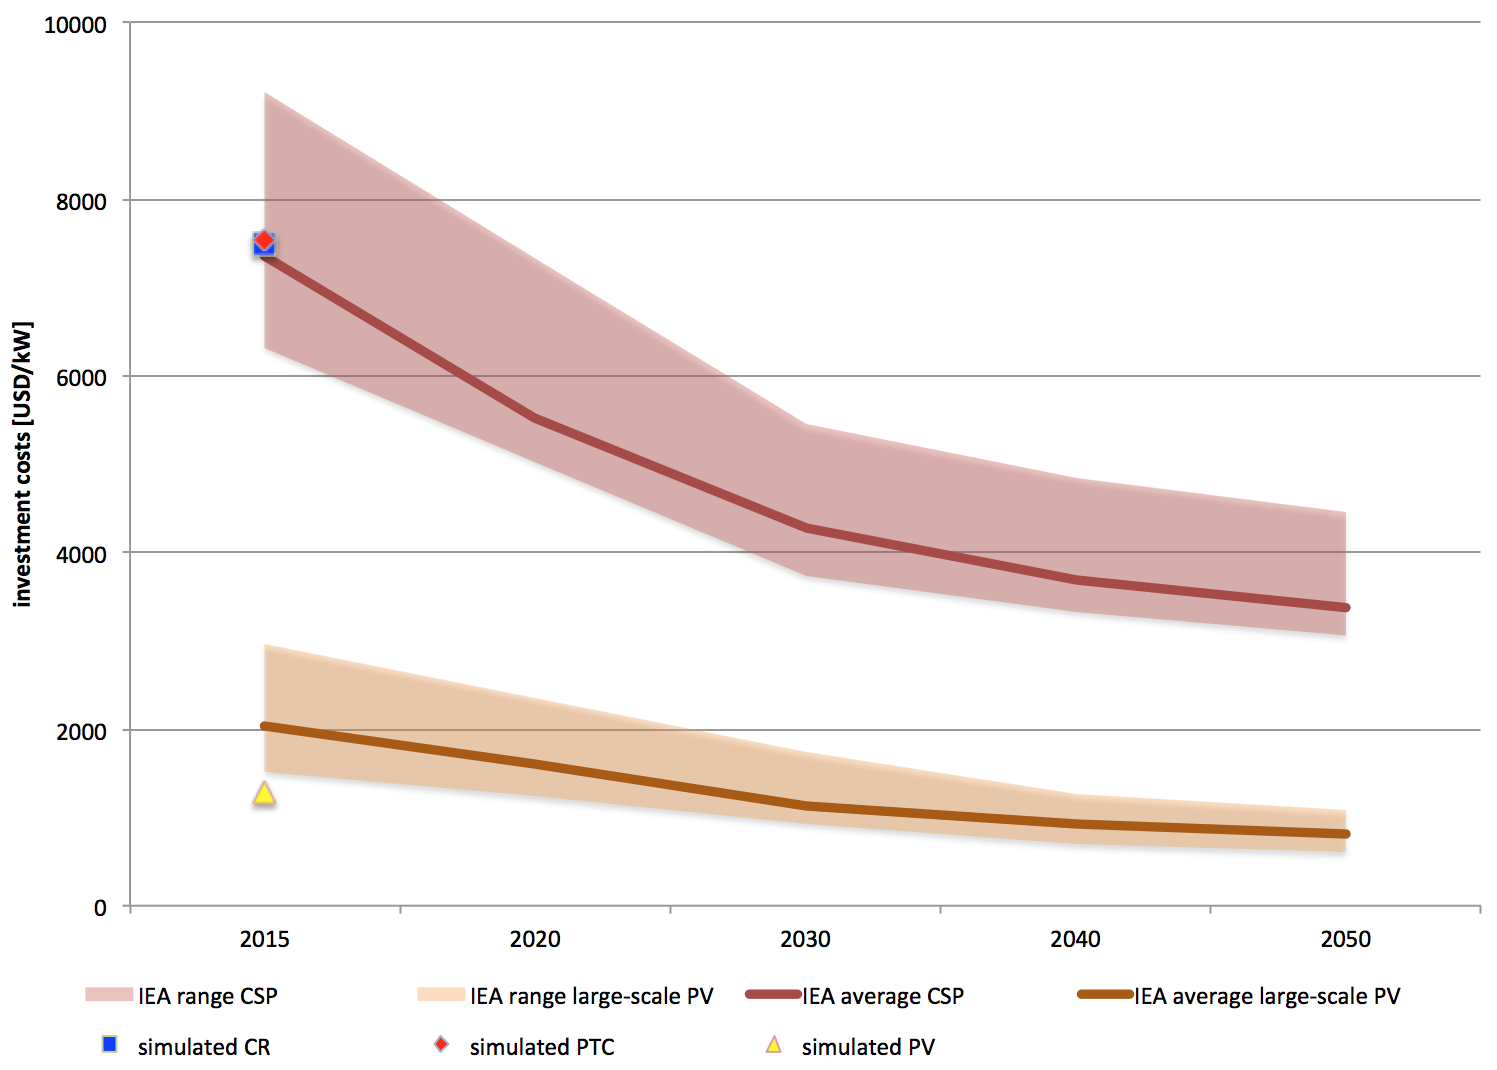
\includegraphics[width=1\linewidth]{FIG/investmentcost}
\caption{Specific investment cost of selected simulated solar power plants and IEA cost forecast.}\label{investmentcost}
\end{figure}
%As it was shown the costs of the PV power plant with EES is dominated by the cost for the EES storage unit. Nevertheless the assumed specific cost of the Li-ion batteries of \SI{300}{USD/kWh}  (Page~\pageref{SUBSUBPVFinancialparameter}) is comparatively optimistic as it can be seen in Figure~\ref{CostofLi-ion}. But in these publication "Rapidly falling costs of battery packs for electric vehicles" it was shown, that the annual cost reductions for battery storage was about \SI{8}{\percent} the past years which led to the current average battery cost for market-leading actors of \SI{300}{USD/kWh} in 2014 and predicts the costs for 2017-2018 at around \SI{230}{USD/kWh} \cite{Nykvist2015}. It can not be assumed that this high annual cost reductions can be retained over the next decades, but storage costs of \SI{200}{USD/kWh} in 2020, as well as \SI{150}{USD/kWh} in 2030 could be feasible, which confirms also other publications \cite{MckinseyQuaterly2012}.

Costs of the \ac{PV} power plant with \ac{EES} are dominated by the cost for the \ac{EES} storage unit. The assumed specific cost of the \ac{li-ion} batteries of \SI{300}{\usd/\kilo\watt\hour} (see page~\pageref{SUBSUBPVFinancialparameter}) is nevertheless comparatively optimistic (Figure~\ref{CostofLi-ion}). In the publication \emph{Rapidly falling costs of battery packs for electric vehicles}, it was shown that cost reductions for battery storage have been \SI{8}{\percent\per\year} in the past, leading to a current average battery cost for market-leading actors of \SI{300}{\usd/\kilo\watt\hour} in 2014. Costs for 2017-2018 were predicted to be at around \SI{230}{\usd/\kilo\watt\hour} \cite{Nykvist2015}. It should not be assumed that such large annual cost reductions can be sustained over the next decades, but storage costs of \SI{200}{\usd/\kilo\watt\hour} by 2020 and \SI{150}{\usd/\kilo\watt\hour} by 2030 appear feasible, a position also held by others \cite{MckinseyQuaterly2012}.

\begin{figure}[htbp]  
\centering
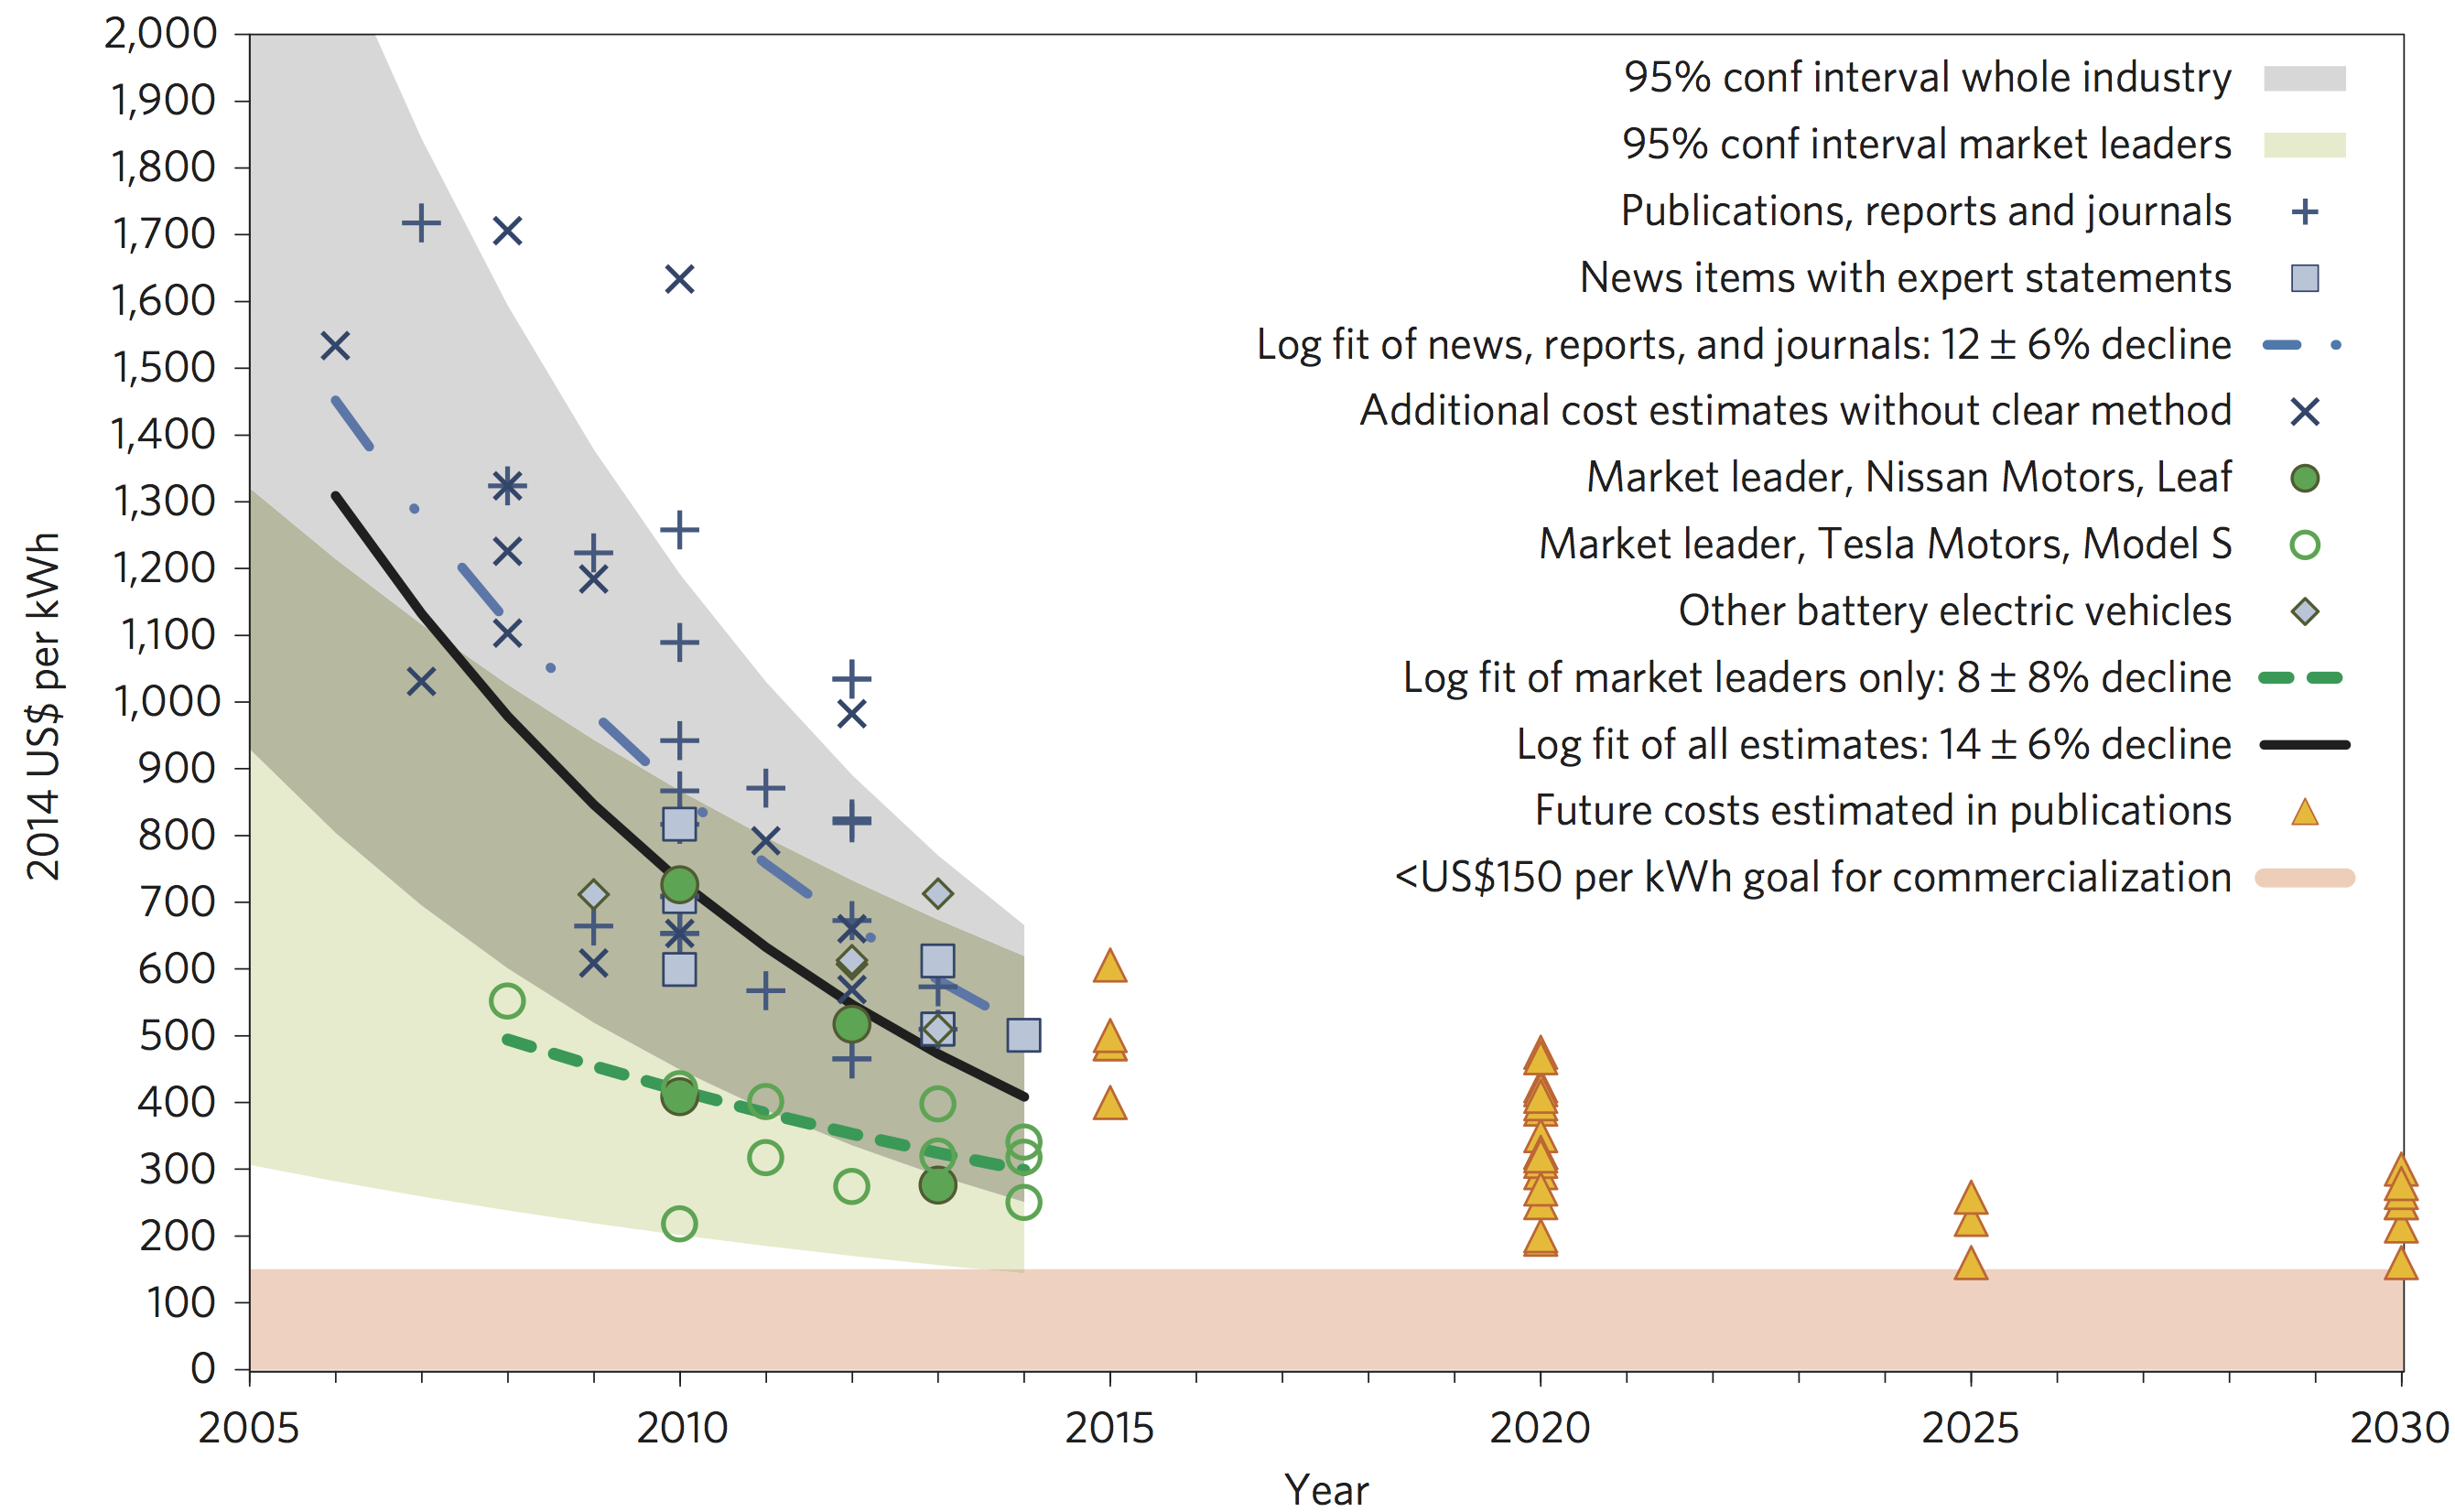
\includegraphics[width=1\linewidth]{FIG/CostofLi-ion}
\caption[Cost of battery packs in battery electric vehicles.]{Cost of battery packs in battery electric vehicles \cite{Nykvist2015}.}\label{CostofLi-ion}
\end{figure}
%The estimated cost reduction for the coming decades of solar power applications and EES was used for a medium-term lookout of the LCOE of the selected simulated systems. Figure~\ref{Costdegrad} shows the expected cost development of the selected solar power plants\footnote{Using the average cost reduction behaviour from \cite{IEA2014c} and assumed storage part cost of the EES of \SI{200}{USD/kWh} in 2020 and \SI{150}{USD/kWh} in 2030.} and the currently expected costs per \si{MWh} for new-built conventional power stations\footnote{Costs per \si{MWh} for conventional new-built options as per IRP Update \cite{CSIR2015a} by using a avarage exchange rate from 2014 of \SI{11.286}{USD/ZAR} \cite{IRS2015}.}. 

These estimated cost degressions in solar power applications and \ac{EES} were used for a forecast of \ac{LCOE} in the selected simulated systems. Figure~\ref{Costdegrad} shows the expected cost evolution of the selected solar power plants\footnote{Using the average projected cost reductions from \cite{IEA2014c} and estimated storage cost of \ac{EES} of \SI{200}{\usd/\kilo\watt\hour} in 2020 and \SI{150}{\usd/\kilo\watt\hour} in 2030.} and the currently expected costs per \si{\mega\watt\hour} for newly-built conventional power stations\footnote{Costs per \si{\mega\watt\hour} for conventional newly-built options as per \ac{IRP} Update \cite{CSIR2015a}, using an average 2014 exchange rate of \SI{11.286}{\usd/\zar} \cite{IRS2015}.}.

%It can be seen that the reduction of the EES storage part effects the electricity price of the PV power plant with EES enormously and could halved the LCOE by 2030. 


%It can be seen that the reduction of the EES storage part effects the electricity price of the PV power plant with EES enormously and could halved there LCOE by 2030. Generally interesting is that a large-scale EES system can compete with the actual electricity costs of a new-build diesel fired OCGT. Also are the estimated electricity cost for a new-built PV system (without EES) almost that cheap than a new-built baseload coal plant. The energy costs\footnote{The electricity costs of the Medupi coal power plant was named with \SI{1.05}{ZAR/kWh} \cite{Nedbank2013} by using a avarage exchange rate from 2014 of \SI{11.286}{USD/ZAR} \cite{IRS2015}.} per \si{MWh} of the currently under constriction situated Medupi coal power plant are with \SI{93}{USD/MWh} actually higher than the cost of the simulated PV system. The decreasing electricity costs of the CSP shows that they can compete in the next decade directly with new-built coal fired mid-merit power plants and new-built combined cycle gas turbine (CCGT). 

Cost reductions of the \ac{EES} storage component affects the electricity price of the \ac{PV} power plant with \ac{EES} enormously and could halve the \ac{LCOE} by 2030. A large-scale \ac{EES} system can compete with the current electricity costs of a new-build diesel fired \ac{OCGT}. The estimated electricity costs for a new-build \ac{PV} system (without \ac{EES}) are almost par with those of a new-build baseload coal plant. The energy costs\footnote{The electricity costs of the Medupi coal power plant was named with \SI{1.05}{\zar/\kilo\watt\hour} \cite{Nedbank2013} by using an average 2014 exchange rate of \SI{11.286}{\usd/\zar} \cite{IRS2015}.} per \si{\mega\watt\hour} of the Medupi coal power plant (currently under construction) are, at \SI{93}{\usd/\mega\watt\hour}, currently higher than the cost of the simulated \ac{PV} system. The decreasing electricity costs of the \ac{CSP} show that they will be able to compete directly with new-built coal fired mid-merit power plants and new-built combined cycle gas turbine (CCGT) within the next decade.
\pagebreak
\begin{figure}[t]  
\centering
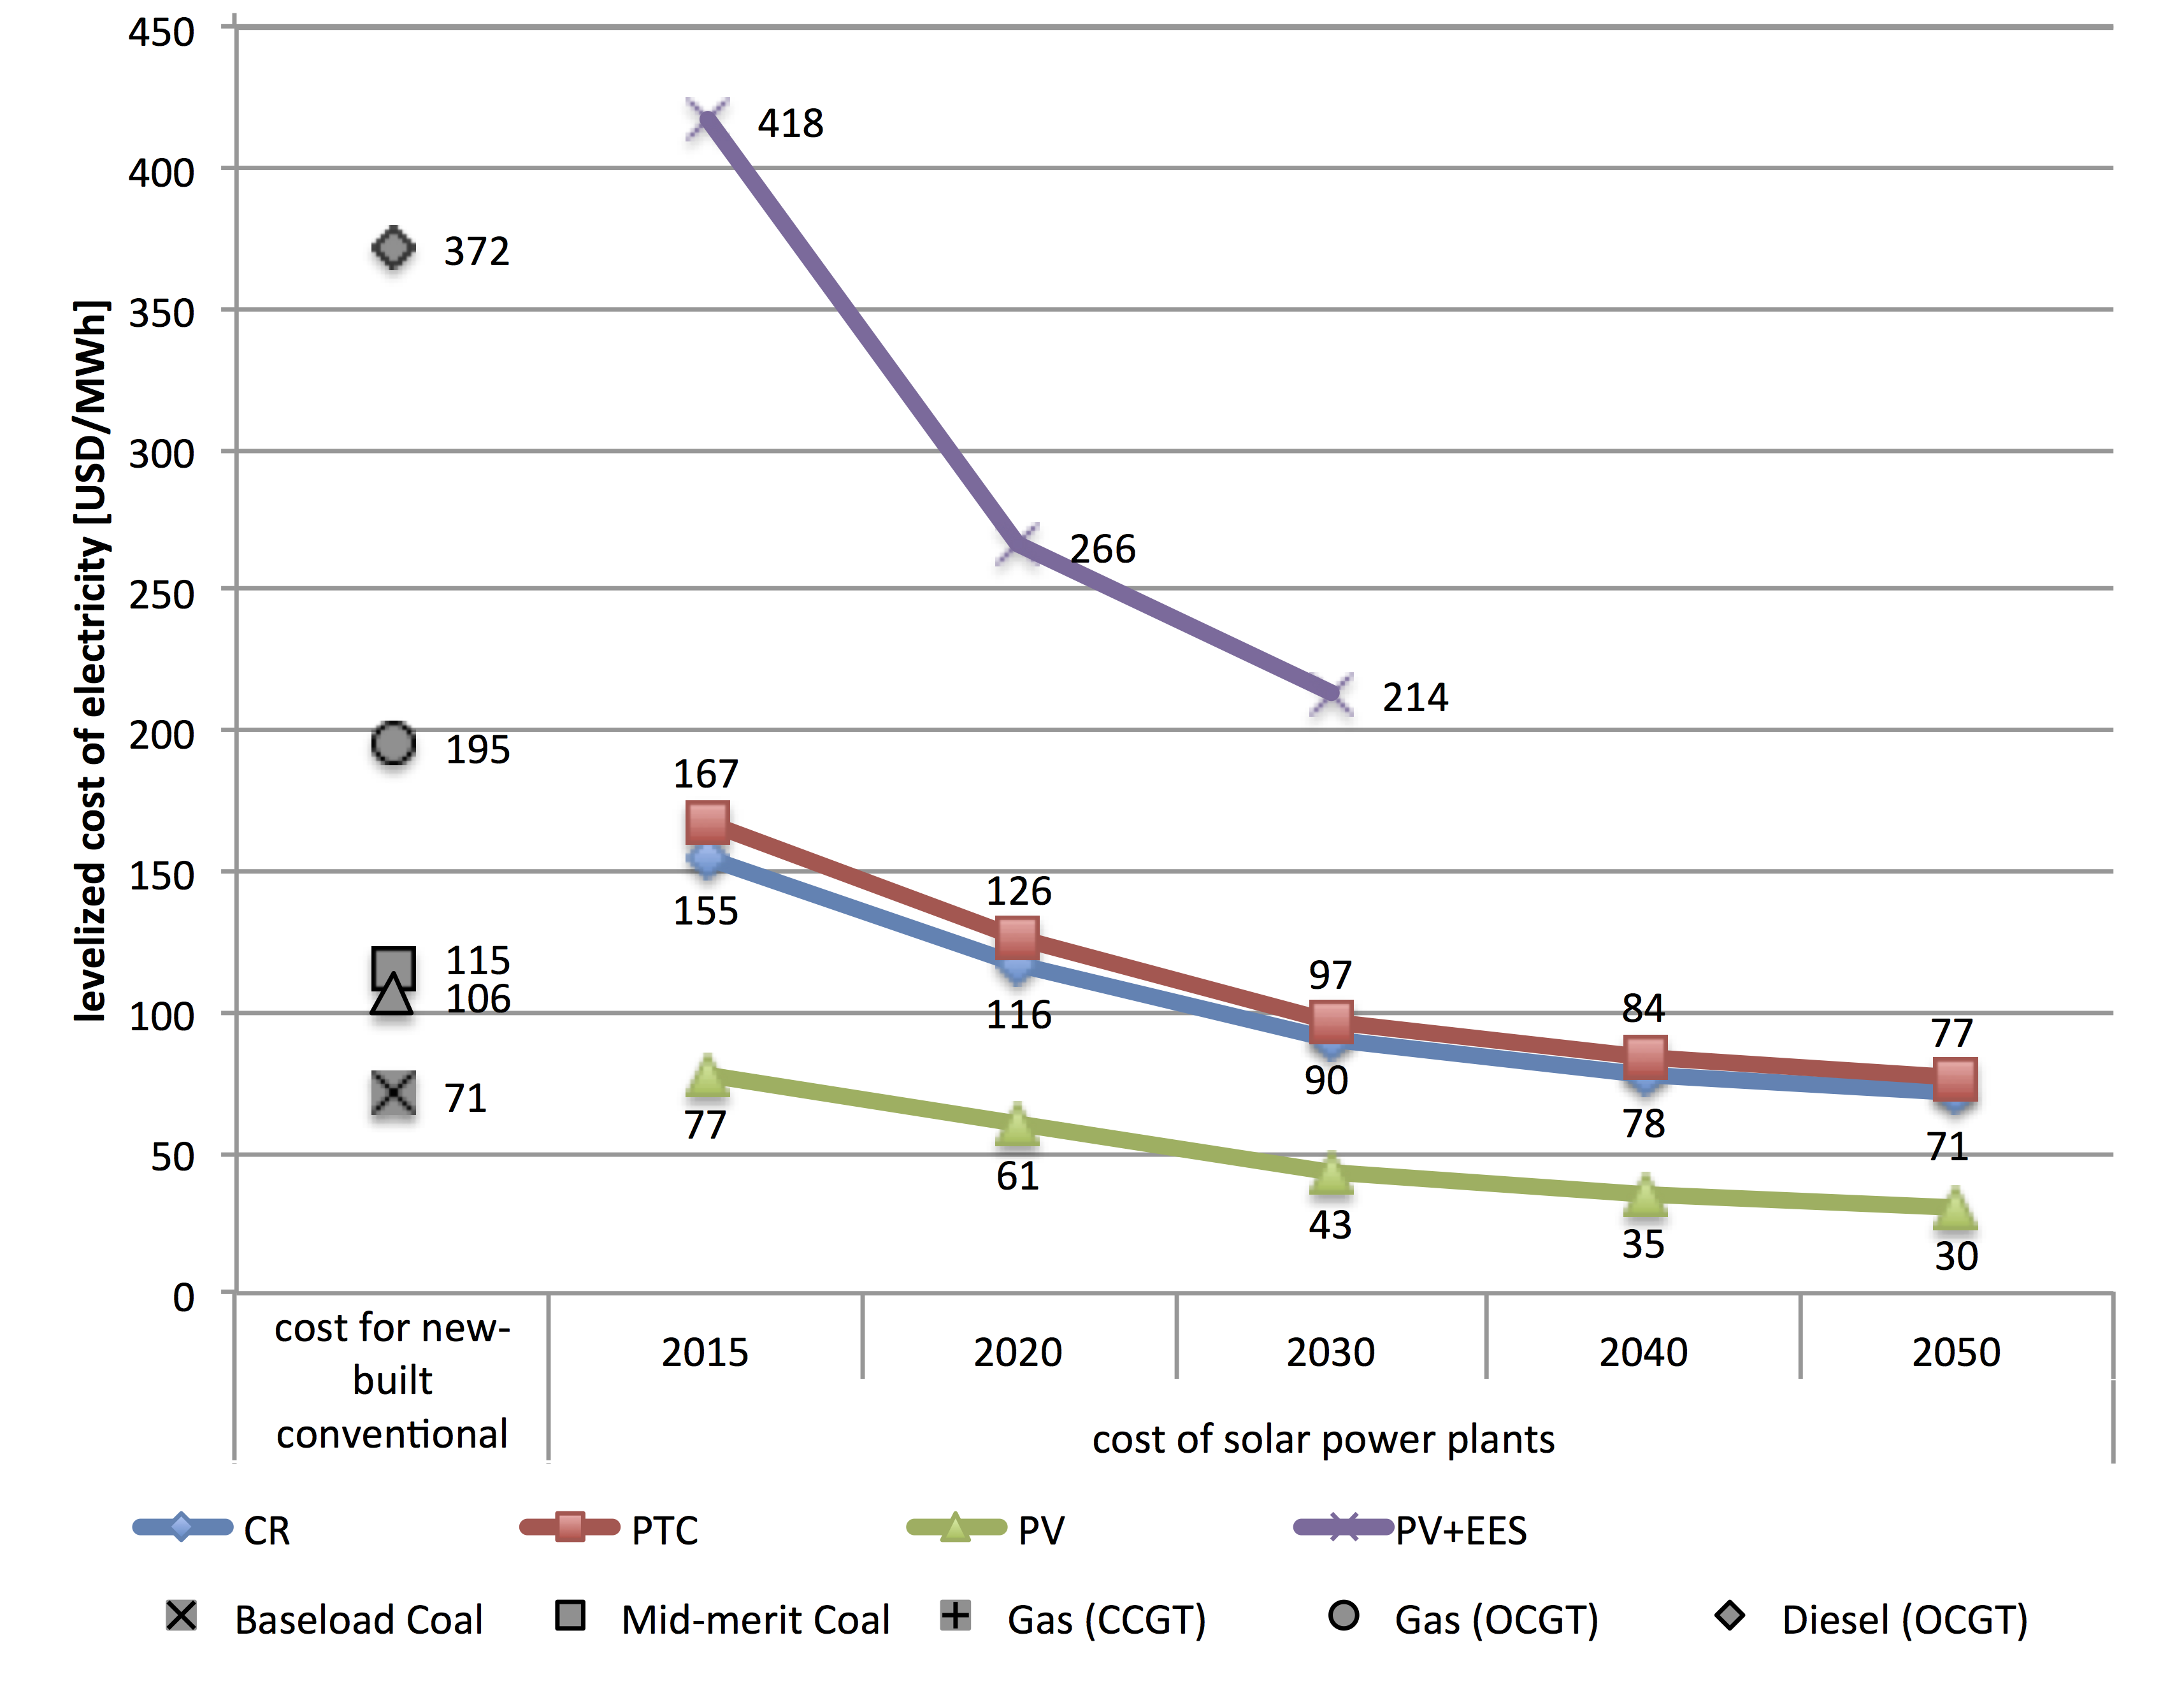
\includegraphics[width=1\linewidth]{FIG/Costdegrad}
\caption[Long-term cost evolution of simulated technologies compared with new-build conventional system costs.]{Long-term cost evolution of simulated technologies compared with new-build conventional system costs.}\label{Costdegrad}
\end{figure}

%It can be seen that for supporting the South African power supply over the full year and especially during the critical evening time as it was defined in Section~\ref{SystemloadinSA} the PV system in combination with a EES based on Li-ion technology is much more expansive than a CR or PTC power plant with TES technology. Therefore it can be said that a flexible power supply based on a PV system is not economically. Also the long-therm cost development for the next decades shows, that this status will not change. Whereas CSP technology can supply in combination with a TES flexible load shapes with economically acceptable costs, which will decrease in the coming years further and getting to more economically than coal fired mid-merit power plants.

Given the objectives defined in Section~\ref{SystemloadinSA}, the \ac{PV} system in combination with an \ac{EES} based on \ac{li-ion} technology is much more expensive than a \ac{CR} or \ac{PTC} power plant with \ac{TES} technology. A flexible power supply based on a \ac{PV} system is not economically viable. The long-term cost evolution for the next decades shows that this will not change. In contrast, \ac{CSP} technology in combination with \ac{TES} can supply variable loads with economically acceptable costs, which should decrease further in the coming years, becoming more economical than coal-fired mid-merit power plants.